\documentclass[11pt,a4paper]{article}
\usepackage[T1]{fontenc}
\usepackage[utf8]{inputenc}
\usepackage{mathptmx}
\usepackage[scaled=0.9]{helvet}
\usepackage{courier}
\usepackage[margin=2.3cm]{geometry}
\usepackage{amsmath,amssymb}
\usepackage{graphicx}
\usepackage{booktabs}
\usepackage{multirow}
\usepackage[font=small,labelfont=bf]{caption}
\usepackage{subcaption}
\usepackage{xcolor}
\usepackage[round,authoryear]{natbib}
\usepackage{microtype}
\usepackage{enumitem}
\usepackage[colorlinks=true,linkcolor=blue!50!black,citecolor=blue!50!black,urlcolor=blue!50!black]{hyperref}
\usepackage{cleveref}

\setlist{nosep,leftmargin=1.4em}
\setlength{\parskip}{0.35em}
\graphicspath{{../figures/}}
% generated by experiments/tables.py
\newcommand{\AbIvfMs}{0.89}
\newcommand{\AbIvfRecall}{0.907}
\newcommand{\AbOldAnchor}{0.058}
\newcommand{\AbOursMs}{0.37}
\newcommand{\AbSFour}{0.863}
\newcommand{\AbSOne}{0.992}
\newcommand{\AbSQuarter}{0.259}
\newcommand{\BvBuilds}{7}
\newcommand{\BvCodeMax}{0.983}
\newcommand{\BvCodeMin}{0.972}
\newcommand{\BvPaperMax}{0.968}
\newcommand{\BvPaperMin}{0.959}
\newcommand{\BvRawMax}{0.997}
\newcommand{\BvRawMin}{0.994}
\newcommand{\CalAttended}{5.1}
\newcommand{\CalKnew}{13.4}
\newcommand{\CfActrRelEight}{0.59\%}
\newcommand{\CfActrRngEight}{0.30\%}
\newcommand{\CfFadeRngEight}{0.36\%}
\newcommand{\CfFastRate}{1.7}
\newcommand{\CfHypRngEight}{0.06\%}
\newcommand{\CuAgeActrHundredK}{80.3}
\newcommand{\CuAgeActrOneM}{0.8}
\newcommand{\CuAgePaperHundredK}{8.9}
\newcommand{\CuAgePaperOneM}{5.9}
\newcommand{\CuFitMsHundredK}{17}
\newcommand{\CuFitMsOneM}{268}
\newcommand{\CuFitRecallHundredK}{0.999}
\newcommand{\CuFitRecallOneM}{0.996}
\newcommand{\CuFrontMax}{26}
\newcommand{\CuFrontMaxOneM}{34}
\newcommand{\CuFrontMin}{1}
\newcommand{\CuFrontMinOneM}{1}
\newcommand{\CuOursDeepHundredK}{0.989}
\newcommand{\CuOursDeepMsHundredK}{1.05}
\newcommand{\CuOursDeepMsOneM}{2.87}
\newcommand{\CuOursDeepOneM}{0.975}
\newcommand{\CuOursMsHundredK}{0.70}
\newcommand{\CuOursMsOneM}{2.40}
\newcommand{\CuOursRecallHundredK}{0.982}
\newcommand{\CuOursRecallOneM}{0.969}
\newcommand{\CuOursSixMsOneM}{1.55}
\newcommand{\CuOursSixRecallOneM}{0.954}
\newcommand{\CuOverlapHundredK}{34\%}
\newcommand{\CuOverlapOneM}{17\%}
\newcommand{\CuREight}{0.988}
\newcommand{\CuRFour}{0.958}
\newcommand{\CuRSix}{0.977}
\newcommand{\CuRTen}{0.991}
\newcommand{\CuRangeEst}{0.982}
\newcommand{\CuRangeExact}{0.990}
\newcommand{\CuRecentHundredK}{5\,963}
\newcommand{\CuRecentOneM}{60\,824}
\newcommand{\CuRecentSixOneM}{19\,059}
\newcommand{\CuRelHundredK}{0.014}
\newcommand{\CuRelOneM}{0.008}
\newcommand{\CuRerankHundredK}{0.085}
\newcommand{\CuRerankKHundredK}{0.438}
\newcommand{\CuRerankKMsHundredK}{2.05}
\newcommand{\CuRerankKMsOneM}{2.77}
\newcommand{\CuRerankKOneM}{0.101}
\newcommand{\CuRerankOneM}{0.030}
\newcommand{\CuSegN}{94\,037}
\newcommand{\CuSegNOneM}{939\,176}
\newcommand{\CuSpeedupOneM}{112}
\newcommand{\GaAgeCodeW}{10.0}
\newcommand{\GaAgePaper}{8.6}
\newcommand{\GaAgeRef}{17.6}
\newcommand{\GaOverlap}{89\%}
\newcommand{\GaOverlapCodeW}{95\%}
\newcommand{\GlCodeRecall}{0.875}
\newcommand{\GlCodeRecallDeep}{0.959}
\newcommand{\GlExactMsOneM}{64.5}
\newcommand{\GlExactMvMsOneM}{46}
\newcommand{\GlN}{1\,000\,000}
\newcommand{\GlOursExactNorm}{0.997}
\newcommand{\GlOursMsOneM}{0.53}
\newcommand{\GlOursRecallDeep}{0.976}
\newcommand{\GlOursRecallOneM}{0.975}
\newcommand{\GlRelonlyRecallOneM}{0.001}
\newcommand{\GlRerankKRecallOneM}{0.040}
\newcommand{\GlRerankRecallHundredK}{0.068}
\newcommand{\GlRerankRecallOneM}{0.006}
\newcommand{\GlRerankRecallTenK}{0.045}
\newcommand{\GlSpeedupMv}{87}
\newcommand{\GlSpeedupOneM}{121}
\newcommand{\HFourMax}{23834}
\newcommand{\HFourMin}{20764}
\newcommand{\HGloveFlat}{5066}
\newcommand{\HGloveHier}{5101}
\newcommand{\HGloveSimpleExtraHi}{34\%}
\newcommand{\HGloveSimpleExtraLo}{27\%}
\newcommand{\HSevenHeurMax}{0.996}
\newcommand{\HSevenSimpleMax}{0.765}
\newcommand{\HThreeBest}{79}
\newcommand{\HThreeBestML}{0.3}
\newcommand{\HThreeDefault}{95}
\newcommand{\HThreeFlat}{211}
\newcommand{\HThreeN}{1\,000\,000}
\newcommand{\HThreeRatio}{2.7}
\newcommand{\HThreeSmallN}{50\,000}
\newcommand{\HThreeSmallRatio}{1.7}
\newcommand{\HvMaxDiff}{0.016}
\newcommand{\HvN}{500\,000}
\newcommand{\HvQpsRatio}{3.2}
\newcommand{\LcDecay}{0.005}
\newcommand{\LcMaxN}{1\,920}
\newcommand{\LcMinN}{1\,308}
\newcommand{\LcOursRecall}{1.000}
\newcommand{\LcRecall}{0.518}
\newcommand{\NeGlA}{0.971}
\newcommand{\NeGlB}{0.982}
\newcommand{\NeGlC}{0.988}
\newcommand{\NeGlCodeA}{0.872}
\newcommand{\NeGlCodeB}{0.879}
\newcommand{\NeGlCodeC}{0.882}
\newcommand{\NeGlCodeD}{0.883}
\newcommand{\NeGlCodeExact}{0.886}
\newcommand{\NeGlCodeMsA}{0.54}
\newcommand{\NeGlCodeMsB}{0.72}
\newcommand{\NeGlCodeMsC}{1.09}
\newcommand{\NeGlCodeMsD}{1.71}
\newcommand{\NeGlD}{0.991}
\newcommand{\NeGlExact}{0.997}
\newcommand{\NeGlMsA}{0.47}
\newcommand{\NeGlMsB}{0.57}
\newcommand{\NeGlMsC}{1.16}
\newcommand{\NeGlMsD}{1.70}
\newcommand{\NeTwA}{0.967}
\newcommand{\NeTwB}{0.970}
\newcommand{\NeTwC}{0.982}
\newcommand{\NeTwCodeA}{0.978}
\newcommand{\NeTwCodeB}{0.984}
\newcommand{\NeTwCodeC}{0.988}
\newcommand{\NeTwCodeD}{0.992}
\newcommand{\NeTwCodeExact}{0.997}
\newcommand{\NeTwCodeMsA}{0.22}
\newcommand{\NeTwCodeMsB}{0.22}
\newcommand{\NeTwCodeMsC}{0.27}
\newcommand{\NeTwCodeMsD}{0.45}
\newcommand{\NeTwD}{0.984}
\newcommand{\NeTwExact}{0.990}
\newcommand{\NeTwMsA}{0.16}
\newcommand{\NeTwMsB}{0.17}
\newcommand{\NeTwMsC}{0.40}
\newcommand{\NeTwMsD}{0.38}
\newcommand{\RsEightFolded}{0.759}
\newcommand{\RsEightFoldedDeep}{0.909}
\newcommand{\RsEightRerank}{0.699}
\newcommand{\RsEightRerankK}{0.954}
\newcommand{\RsHalfMin}{0.924}
\newcommand{\RsLowFoldedMin}{0.983}
\newcommand{\RsLowRerankMax}{0.245}
\newcommand{\RsSixteenFolded}{0.695}
\newcommand{\RsSixteenFoldedDeep}{0.868}
\newcommand{\RsSixteenRerank}{0.848}
\newcommand{\RsSixteenRerankK}{0.983}
\newcommand{\TNinetyExAtt}{5.8}
\newcommand{\TNinetyExAware}{13.1}
\newcommand{\TNinetyExRecall}{1.000}
\newcommand{\TNinetyExRecalled}{10.8}
\newcommand{\TNinetyFoAtt}{5.9}
\newcommand{\TNinetyFoAware}{13.2}
\newcommand{\TNinetyFoMaxDiff}{2}
\newcommand{\TNinetyFoRecall}{0.999}
\newcommand{\TNinetyFoRecallEnd}{1.00}
\newcommand{\TNinetyFoRecalled}{10.9}
\newcommand{\TNinetyFoSame}{26}
\newcommand{\TNinetyNrAtt}{3.8}
\newcommand{\TNinetyNrAttP}{0.0003}
\newcommand{\TNinetyNrAware}{8.3}
\newcommand{\TNinetyNrAwareP}{2.5e-06}
\newcommand{\TNinetyNrRecall}{0.502}
\newcommand{\TNinetyNrRecalled}{6.8}
\newcommand{\TNinetyNrRecalledP}{5.2e-06}
\newcommand{\TNinetyReAtt}{6.8}
\newcommand{\TNinetyReAttHolm}{0.37}
\newcommand{\TNinetyReAware}{15.2}
\newcommand{\TNinetyReAwareHolm}{0.011}
\newcommand{\TNinetyReRecall}{0.487}
\newcommand{\TNinetyReRecallEnd}{0.32}
\newcommand{\TNinetyReRecalled}{13.3}
\newcommand{\TNinetyReRecalledHolm}{0.0063}
\newcommand{\TNinetyRelAtt}{3.3}
\newcommand{\TNinetyRelAware}{8.2}
\newcommand{\TNinetyRelRecall}{0.366}
\newcommand{\TNinetyRelRecallEnd}{0.26}
\newcommand{\TNinetyRelRecalled}{5.4}
\newcommand{\TNinetySeeds}{30}
\newcommand{\TRelDropAttHi}{45\%}
\newcommand{\TRelDropAttLo}{33\%}
\newcommand{\TRelDropAwareHi}{43\%}
\newcommand{\TRelDropAwareLo}{38\%}
\newcommand{\TSevenExAtt}{5.0}
\newcommand{\TSevenExAware}{11.7}
\newcommand{\TSevenExRecall}{1.000}
\newcommand{\TSevenExRecalled}{10.1}
\newcommand{\TSevenFoAtt}{5.0}
\newcommand{\TSevenFoAware}{11.7}
\newcommand{\TSevenFoMaxDiff}{0}
\newcommand{\TSevenFoRecall}{1.000}
\newcommand{\TSevenFoRecalled}{10.1}
\newcommand{\TSevenFoSame}{30}
\newcommand{\TSevenReAtt}{4.9}
\newcommand{\TSevenReAttHolm}{1}
\newcommand{\TSevenReAware}{11.2}
\newcommand{\TSevenReAwareHolm}{0.037}
\newcommand{\TSevenReRecall}{0.876}
\newcommand{\TSevenReRecalled}{9.7}
\newcommand{\TSevenReRecalledHolm}{0.29}
\newcommand{\TSevenRelAtt}{3.4}
\newcommand{\TSevenRelAware}{7.3}
\newcommand{\TSevenRelRecall}{0.637}
\newcommand{\TSevenRelRecalled}{6.3}
\newcommand{\TSevenSeeds}{30}
\newcommand{\TThirtyExAtt}{5.0}
\newcommand{\TThirtyExAware}{11.7}
\newcommand{\TThirtyExRecall}{1.000}
\newcommand{\TThirtyExRecalled}{9.5}
\newcommand{\TThirtyFoAtt}{5.0}
\newcommand{\TThirtyFoAware}{11.7}
\newcommand{\TThirtyFoMaxDiff}{0}
\newcommand{\TThirtyFoRecall}{1.000}
\newcommand{\TThirtyFoRecalled}{9.5}
\newcommand{\TThirtyFoSame}{30}
\newcommand{\TThirtyNrAtt}{3.3}
\newcommand{\TThirtyNrAttP}{1.4e-05}
\newcommand{\TThirtyNrAware}{7.0}
\newcommand{\TThirtyNrAwareP}{1.6e-06}
\newcommand{\TThirtyNrRecall}{0.679}
\newcommand{\TThirtyNrRecalled}{5.9}
\newcommand{\TThirtyNrRecalledP}{3.6e-06}
\newcommand{\TThirtyReAtt}{4.9}
\newcommand{\TThirtyReAttHolm}{1}
\newcommand{\TThirtyReAware}{10.9}
\newcommand{\TThirtyReAwareHolm}{0.37}
\newcommand{\TThirtyReRecall}{0.681}
\newcommand{\TThirtyReRecalled}{9.1}
\newcommand{\TThirtyReRecalledHolm}{0.79}
\newcommand{\TThirtyRelAtt}{2.7}
\newcommand{\TThirtyRelAware}{6.7}
\newcommand{\TThirtyRelRecall}{0.488}
\newcommand{\TThirtyRelRecalled}{4.9}
\newcommand{\TThirtySeeds}{30}
\newcommand{\TZeroExAtt}{5.5}
\newcommand{\TZeroExAware}{12.6}
\newcommand{\TZeroExRecall}{1.000}
\newcommand{\TZeroExRecalled}{10.7}
\newcommand{\TZeroFoAtt}{5.5}
\newcommand{\TZeroFoAware}{12.6}
\newcommand{\TZeroFoMaxDiff}{0}
\newcommand{\TZeroFoRecall}{1.000}
\newcommand{\TZeroFoRecalled}{10.7}
\newcommand{\TZeroFoSame}{30}
\newcommand{\TZeroReAtt}{5.5}
\newcommand{\TZeroReAware}{12.6}
\newcommand{\TZeroReRecall}{0.995}
\newcommand{\TZeroReRecalled}{10.7}
\newcommand{\TZeroRelAtt}{5.4}
\newcommand{\TZeroRelAware}{11.9}
\newcommand{\TZeroRelRecall}{0.872}
\newcommand{\TZeroRelRecalled}{10.2}
\newcommand{\TZeroSeeds}{30}
\newcommand{\TcDiagLastMaxRet}{656}
\newcommand{\TcDiagLastNewHour}{0.70}
\newcommand{\TcDiagLastPerMem}{5.3}
\newcommand{\TcDiagLastTopShare}{64\%}
\newcommand{\TcDiagLogMaxRet}{692}
\newcommand{\TcDiagLogNewHour}{0.49}
\newcommand{\TcDiagLogPerMem}{5.3}
\newcommand{\TcDiagLogTopShare}{78\%}
\newcommand{\TcDiagSeeds}{5}
\newcommand{\TcDiagUsesMaxRet}{735}
\newcommand{\TcDiagUsesNewHour}{0.02}
\newcommand{\TcDiagUsesPerMem}{5.3}
\newcommand{\TcDiagUsesTopShare}{82\%}
\newcommand{\TcNinetyExMs}{0.06}
\newcommand{\TcNinetyExpAtt}{5.8}
\newcommand{\TcNinetyExpAware}{13.1}
\newcommand{\TcNinetyExpRecalled}{10.8}
\newcommand{\TcNinetyFoMs}{2.30}
\newcommand{\TcNinetyLastExAtt}{6.5}
\newcommand{\TcNinetyLastExAware}{15.2}
\newcommand{\TcNinetyLastExRecall}{1.000}
\newcommand{\TcNinetyLastExRecallFour}{1.0000}
\newcommand{\TcNinetyLastExRecalled}{12.4}
\newcommand{\TcNinetyLastFoAtt}{6.4}
\newcommand{\TcNinetyLastFoAttHolm}{1}
\newcommand{\TcNinetyLastFoAware}{15.1}
\newcommand{\TcNinetyLastFoAwareHolm}{1}
\newcommand{\TcNinetyLastFoMaxDiff}{2}
\newcommand{\TcNinetyLastFoRecall}{1.000}
\newcommand{\TcNinetyLastFoRecallFour}{0.9996}
\newcommand{\TcNinetyLastFoRecalled}{12.3}
\newcommand{\TcNinetyLastFoRecalledHolm}{1}
\newcommand{\TcNinetyLastFoSame}{26}
\newcommand{\TcNinetyLastReAtt}{6.8}
\newcommand{\TcNinetyLastReAttHolm}{1}
\newcommand{\TcNinetyLastReAware}{15.2}
\newcommand{\TcNinetyLastReAwareHolm}{1}
\newcommand{\TcNinetyLastReRecall}{0.536}
\newcommand{\TcNinetyLastReRecallFour}{0.5361}
\newcommand{\TcNinetyLastReRecalled}{13.3}
\newcommand{\TcNinetyLastReRecalledHolm}{0.84}
\newcommand{\TcNinetyLastSeeds}{30}
\newcommand{\TcNinetyLastVsExpAttHolm}{0.0016}
\newcommand{\TcNinetyLastVsExpAwareHolm}{0.00019}
\newcommand{\TcNinetyLastVsExpRecalledHolm}{0.00049}
\newcommand{\TcNinetyLastVsExpSeeds}{30}
\newcommand{\TcNinetyLogExAtt}{1.8}
\newcommand{\TcNinetyLogExAware}{9.8}
\newcommand{\TcNinetyLogExRecall}{1.000}
\newcommand{\TcNinetyLogExRecallFour}{1.0000}
\newcommand{\TcNinetyLogExRecalled}{2.8}
\newcommand{\TcNinetyLogFoAttHolm}{1}
\newcommand{\TcNinetyLogFoAwareHolm}{1}
\newcommand{\TcNinetyLogFoRecalledHolm}{1}
\newcommand{\TcNinetyLogReAttHolm}{1}
\newcommand{\TcNinetyLogReAwareHolm}{1}
\newcommand{\TcNinetyLogReRecalledHolm}{1}
\newcommand{\TcNinetyLogVsExpAttHolm}{5e-05}
\newcommand{\TcNinetyLogVsExpAwareHolm}{6.7e-05}
\newcommand{\TcNinetyLogVsExpRecalledHolm}{2.9e-05}
\newcommand{\TcNinetyLogVsExpSeeds}{30}
\newcommand{\TcNinetyUsesExAtt}{1.2}
\newcommand{\TcNinetyUsesExAware}{9.2}
\newcommand{\TcNinetyUsesExRecall}{1.000}
\newcommand{\TcNinetyUsesExRecallFour}{1.0000}
\newcommand{\TcNinetyUsesExRecalled}{1.4}
\newcommand{\TcNinetyUsesFoAtt}{1.2}
\newcommand{\TcNinetyUsesFoAttHolm}{1}
\newcommand{\TcNinetyUsesFoAware}{9.1}
\newcommand{\TcNinetyUsesFoAwareHolm}{1}
\newcommand{\TcNinetyUsesFoMaxDiff}{2}
\newcommand{\TcNinetyUsesFoRecall}{1.000}
\newcommand{\TcNinetyUsesFoRecallFour}{0.9996}
\newcommand{\TcNinetyUsesFoRecalled}{1.4}
\newcommand{\TcNinetyUsesFoRecalledHolm}{1}
\newcommand{\TcNinetyUsesFoSame}{27}
\newcommand{\TcNinetyUsesReAtt}{5.9}
\newcommand{\TcNinetyUsesReAttHolm}{3.9e-05}
\newcommand{\TcNinetyUsesReAware}{15.2}
\newcommand{\TcNinetyUsesReAwareHolm}{5.5e-05}
\newcommand{\TcNinetyUsesReRecall}{0.456}
\newcommand{\TcNinetyUsesReRecallFour}{0.4556}
\newcommand{\TcNinetyUsesReRecalled}{11.5}
\newcommand{\TcNinetyUsesReRecalledHolm}{3.9e-05}
\newcommand{\TcNinetyUsesSeeds}{30}
\newcommand{\TcNinetyUsesVsExpAttHolm}{3.6e-05}
\newcommand{\TcNinetyUsesVsExpAwareHolm}{6.7e-05}
\newcommand{\TcNinetyUsesVsExpRecalledHolm}{2.9e-05}
\newcommand{\TcNinetyUsesVsExpSeeds}{30}
\newcommand{\TcRuns}{630}
\newcommand{\TcShapeActrFive}{0.40}
\newcommand{\TcShapeActrThirtyFive}{0.15}
\newcommand{\TcShapeExpFive}{0.98}
\newcommand{\TcShapeExpThirtyFive}{0.84}
\newcommand{\TcThirtyExMs}{0.04}
\newcommand{\TcThirtyExpAtt}{5.0}
\newcommand{\TcThirtyExpAware}{11.7}
\newcommand{\TcThirtyExpRecalled}{9.5}
\newcommand{\TcThirtyFoMs}{1.05}
\newcommand{\TcThirtyLastExAtt}{5.1}
\newcommand{\TcThirtyLastExAware}{12.1}
\newcommand{\TcThirtyLastExRecall}{1.000}
\newcommand{\TcThirtyLastExRecallFour}{1.0000}
\newcommand{\TcThirtyLastExRecalled}{9.8}
\newcommand{\TcThirtyLastFoAtt}{5.1}
\newcommand{\TcThirtyLastFoAttHolm}{1}
\newcommand{\TcThirtyLastFoAware}{12.1}
\newcommand{\TcThirtyLastFoAwareHolm}{1}
\newcommand{\TcThirtyLastFoMaxDiff}{0}
\newcommand{\TcThirtyLastFoRecall}{1.000}
\newcommand{\TcThirtyLastFoRecallFour}{0.9995}
\newcommand{\TcThirtyLastFoRecalled}{9.8}
\newcommand{\TcThirtyLastFoRecalledHolm}{1}
\newcommand{\TcThirtyLastFoSame}{30}
\newcommand{\TcThirtyLastReAtt}{4.9}
\newcommand{\TcThirtyLastReAttHolm}{0.37}
\newcommand{\TcThirtyLastReAware}{10.9}
\newcommand{\TcThirtyLastReAwareHolm}{0.0056}
\newcommand{\TcThirtyLastReRecall}{0.703}
\newcommand{\TcThirtyLastReRecallFour}{0.7030}
\newcommand{\TcThirtyLastReRecalled}{9.1}
\newcommand{\TcThirtyLastReRecalledHolm}{0.048}
\newcommand{\TcThirtyLastSeeds}{30}
\newcommand{\TcThirtyLastVsExpAttHolm}{0.2}
\newcommand{\TcThirtyLastVsExpAwareHolm}{0.2}
\newcommand{\TcThirtyLastVsExpRecalledHolm}{0.2}
\newcommand{\TcThirtyLastVsExpSeeds}{30}
\newcommand{\TcThirtyLogExAtt}{3.9}
\newcommand{\TcThirtyLogExAware}{10.0}
\newcommand{\TcThirtyLogExRecall}{1.000}
\newcommand{\TcThirtyLogExRecallFour}{1.0000}
\newcommand{\TcThirtyLogExRecalled}{7.1}
\newcommand{\TcThirtyLogFoAttHolm}{1}
\newcommand{\TcThirtyLogFoAwareHolm}{1}
\newcommand{\TcThirtyLogFoRecalledHolm}{1}
\newcommand{\TcThirtyLogReAttHolm}{1}
\newcommand{\TcThirtyLogReAwareHolm}{1}
\newcommand{\TcThirtyLogReRecalledHolm}{1}
\newcommand{\TcThirtyLogVsExpAttHolm}{0.00057}
\newcommand{\TcThirtyLogVsExpAwareHolm}{0.00058}
\newcommand{\TcThirtyLogVsExpRecalledHolm}{0.00022}
\newcommand{\TcThirtyLogVsExpSeeds}{30}
\newcommand{\TcThirtyUsesExAtt}{3.3}
\newcommand{\TcThirtyUsesExAware}{9.5}
\newcommand{\TcThirtyUsesExRecall}{1.000}
\newcommand{\TcThirtyUsesExRecallFour}{1.0000}
\newcommand{\TcThirtyUsesExRecalled}{5.8}
\newcommand{\TcThirtyUsesFoAtt}{3.2}
\newcommand{\TcThirtyUsesFoAttHolm}{1}
\newcommand{\TcThirtyUsesFoAware}{9.3}
\newcommand{\TcThirtyUsesFoAwareHolm}{1}
\newcommand{\TcThirtyUsesFoMaxDiff}{4}
\newcommand{\TcThirtyUsesFoRecall}{1.000}
\newcommand{\TcThirtyUsesFoRecallFour}{0.9998}
\newcommand{\TcThirtyUsesFoRecalled}{5.6}
\newcommand{\TcThirtyUsesFoRecalledHolm}{1}
\newcommand{\TcThirtyUsesFoSame}{27}
\newcommand{\TcThirtyUsesReAtt}{4.8}
\newcommand{\TcThirtyUsesReAttHolm}{0.00017}
\newcommand{\TcThirtyUsesReAware}{10.9}
\newcommand{\TcThirtyUsesReAwareHolm}{0.018}
\newcommand{\TcThirtyUsesReRecall}{0.601}
\newcommand{\TcThirtyUsesReRecallFour}{0.6013}
\newcommand{\TcThirtyUsesReRecalled}{9.0}
\newcommand{\TcThirtyUsesReRecalledHolm}{0.00011}
\newcommand{\TcThirtyUsesSeeds}{30}
\newcommand{\TcThirtyUsesVsExpAttHolm}{6.7e-05}
\newcommand{\TcThirtyUsesVsExpAwareHolm}{0.00029}
\newcommand{\TcThirtyUsesVsExpRecalledHolm}{3.6e-05}
\newcommand{\TcThirtyUsesVsExpSeeds}{30}
\newcommand{\TownRuns}{1\,350}
\newcommand{\TrFoMaxDiff}{0}
\newcommand{\TrFoRecallFour}{0.9985}
\newcommand{\TrFoSame}{30}
\newcommand{\TrFoSeeds}{30}
\newcommand{\TrSeeds}{30}
\newcommand{\TrVsLastAttHolm}{0.0029}
\newcommand{\TrVsLastAwareHolm}{0.83}
\newcommand{\TrVsLastRecalledHolm}{0.00097}
\newcommand{\TrWOneNinetyAtt}{2.1}
\newcommand{\TrWOneNinetyAware}{10.8}
\newcommand{\TrWOneNinetyRecalled}{3.4}
\newcommand{\TrWOneThirtyAtt}{4.2}
\newcommand{\TrWOneThirtyAware}{10.8}
\newcommand{\TrWOneThirtyRecalled}{8.0}
\newcommand{\TrWThreeHundredthNinetyAtt}{5.6}
\newcommand{\TrWThreeHundredthNinetyAware}{15.0}
\newcommand{\TrWThreeHundredthNinetyRecalled}{10.4}
\newcommand{\TrWThreeHundredthThirtyAtt}{5.0}
\newcommand{\TrWThreeHundredthThirtyAware}{11.8}
\newcommand{\TrWThreeHundredthThirtyRecalled}{9.6}
\newcommand{\TrWThreeNinetyAtt}{1.3}
\newcommand{\TrWThreeNinetyAware}{9.4}
\newcommand{\TrWThreeNinetyRecalled}{1.7}
\newcommand{\TrWThreeThirtyAtt}{3.5}
\newcommand{\TrWThreeThirtyAware}{9.7}
\newcommand{\TrWThreeThirtyRecalled}{6.4}
\newcommand{\TwExactMs}{5.12}
\newcommand{\TwIpDeep}{0.963}
\newcommand{\TwIvfCodeRecall}{0.800}
\newcommand{\TwIvfMs}{0.31}
\newcommand{\TwIvfRecall}{0.996}
\newcommand{\TwLtwoDeep}{0.981}
\newcommand{\TwN}{126\,454}
\newcommand{\TwOldAnchor}{0.202}
\newcommand{\TwOursCodeRecall}{0.978}
\newcommand{\TwOursExactNorm}{0.990}
\newcommand{\TwOursMs}{0.16}
\newcommand{\TwOursRecall}{0.959}
\newcommand{\TwRelonlyRecall}{0.042}
\newcommand{\TwRerankRecall}{0.277}
\newcommand{\TwSimExactMs}{1.77}
\newcommand{\TwSimFoldedMs}{1.90}
\newcommand{\TwSimMemories}{5\,041}

\IfFileExists{generated/fallbacks.tex}{% placeholders for numbers not generated yet
\providecommand{\AbOldAnchor}{\textbf{??}}
\providecommand{\AbSFour}{\textbf{??}}
\providecommand{\AbSOne}{\textbf{??}}
\providecommand{\AbSQuarter}{\textbf{??}}
\providecommand{\GlExactMsOneM}{\textbf{??}}
\providecommand{\GlOursMsOneM}{\textbf{??}}
\providecommand{\GlOursRecallOneM}{\textbf{??}}
\providecommand{\GlRelonlyRecallOneM}{\textbf{??}}
\providecommand{\GlRerankKRecallOneM}{\textbf{??}}
\providecommand{\GlRerankRecallOneM}{\textbf{??}}
\providecommand{\GlRerankRecallTenK}{\textbf{??}}
\providecommand{\GlSpeedupOneM}{\textbf{??}}
\providecommand{\HvMaxDiff}{\textbf{??}}
\providecommand{\HvN}{\textbf{??}}
\providecommand{\HvQpsRatio}{\textbf{??}}
\providecommand{\RsHalfMin}{\textbf{??}}
\providecommand{\TwN}{\textbf{??}}
\providecommand{\TwOursRecall}{\textbf{??}}
\providecommand{\TwRerankRecall}{\textbf{??}}
}{}

\newcommand{\code}[1]{\texttt{#1}}
\newcommand{\rec}{\mathrm{rec}}
\newcommand{\imp}{\mathrm{imp}}
\newcommand{\rel}{\mathrm{rel}}

\title{\textbf{When the Index Shapes the Agent:\\ Exact Memory Retrieval for Generative Agents with HNSW}\\[0.4em]
\large An extension of the seminar presentation on \citet{malkov2020hnsw}}
\author{Colceriu Mihai Bogdan\\[0.2em]
\small Master in Software Engineering, Technical University of Cluj-Napoca\\
\small Intelligent Agent Systems (Sisteme de agenți inteligenți), 2026--2027}
\date{}

\begin{document}
\maketitle

\begin{abstract}
\noindent Generative agents \citep{park2023generative} decide what to recall by scoring every memory with a weighted sum of recency, importance and relevance. In practice the memories sit in a vector index such as HNSW \citep{malkov2020hnsw}, the article presented at the seminar. A vector index answers a single question: which stored vectors are most similar to the query. Agent frameworks therefore fetch the $K$ most similar memories and re-rank them by the full score, so a memory that is recent or important but not similar enough is never considered. This report first reimplements HNSW from the paper's pseudocode, checks it against the authors' library and repeats the paper's parameter study: the hierarchy pays off in low dimensions, while on clustered and real data the neighbour-selection heuristic matters more. Because recency decays exponentially, the agents' score is an inner product between augmented vectors, an identity that \citet{wei2026tango} have also published for similarity and freshness. A memory store built on it adds what agents need: the importance term, the paper's min-max normalisation, refresh on every access and time-anchored segments that keep the coordinates bounded. With one million memories it keeps recall@10 at \GlOursRecallOneM{} (against \GlRerankRecallOneM{} for the re-ranking used by LangChain) while answering a query roughly a hundred times faster than a linear scan. The report then goes beyond the exponential. Forgetting curves from memory research, such as ACT-R's power law summed over every use of a memory, are close to a sum of a few exponentials, so they too become a single inner-product search: eight extra coordinates follow ACT-R's curve within \CfActrRngEight{} of its range, and the store returns \CuOursRecallOneM{} of the true top-10 among one million memories in \CuOursMsOneM{} ms, where re-ranking returns \CuRerankOneM{}. In a closed-loop simulation of 25 agents calibrated to the paper's party scenario, the folded stores reproduce the behaviour of exact retrieval under both the exponential and ACT-R's curve, while plain similarity search cuts the spread of the invitation by about 40\% in towns older than a week. The simulation also shows that counting every retrieval as a use, as ACT-R's base-level learning does, lets the most retrieved memories crowd out new ones, with or without ACT-R's logarithm. Finally, running the public Generative Agents code shows that its recency term is computed from ranks sorted in the wrong direction, so the memory accessed longest ago receives the highest recency score.
\end{abstract}

\section{Introduction}

Agents built on language models need a memory that outlives the context window. The usual design keeps a stream of natural-language records, embeds each one as a vector and retrieves the records that matter for the current situation \citep{lewis2020rag,wang2024survey}. Generative agents \citep{park2023generative} made the retrieval rule explicit: a memory is worth recalling if it was accessed recently, if it is important and if it is relevant to the query. The three terms are added after min-max scaling.

The index underneath is very often a graph built with HNSW \citep{malkov2020hnsw}. It finds the stored vectors most similar to a query in roughly logarithmic time, but it knows nothing about recency or importance. Frameworks work around this by fetching more candidates than they need and re-ranking them. LangChain's \code{TimeWeightedVectorStoreRetriever} \citep{langchain_twr}, for example, fetches 100 documents by similarity, adds the most recently created ones and returns the best $k$ under the combined score. A memory outside this candidate set is never scored, however recent or important it is. As the memory grows, the candidates cover a shrinking fraction of it. Nothing tells the agent that it is now retrieving something different from what its retrieval rule describes.

This report starts from the HNSW article and asks whether the index itself can answer the agent's real question. It can. The reduction is exact, so the only approximation left is the index's own. The contributions are the following.
\begin{enumerate}
\item A reimplementation of HNSW from Algorithms 1--5 of the paper, validated against hnswlib and used to repeat the paper's parameter study on synthetic data and on GloVe vectors (\cref{sec:hnsw}).
\item A reduction of the Generative Agents score to maximum inner product search (MIPS), obtained by combining forward decay \citep{cormode2009forward} with an inner-product HNSW index, together with a memory store that makes it practical: bounded coordinates, refresh-on-access, min-max normalisation and a replacement for LangChain's retriever with the same scoring rule (\cref{sec:fold}).
\item An extension to forgetting curves from memory research, such as ACT-R's power law summed over every use of a memory, which a few exponentials approximate closely and which therefore also become a single inner-product search. The town shows that counting every retrieval as a use locks an agent's memory in, with or without ACT-R's logarithm (\cref{sec:curves}).
\item An evaluation on up to one million memories (\cref{sec:static,sec:curves}) and in Willowbrook, a closed-loop simulation of 25 agents calibrated to reproduce the information diffusion reported by \citet{park2023generative} (\cref{sec:town,sec:curves}).
\item A check of the public Generative Agents code, which computes recency differently from the paper (\cref{sec:reference}).
\end{enumerate}
The individual ingredients of the second contribution are known. The factorisation of exponential decay into a query part and an item part is the basis of forward decay in stream processing. Graph indexes for inner products were studied by \citet{morozov2018ipnsw}. While this report was being written, \citet{wei2026tango} published the same reduction for a score of similarity and exponential freshness, together with a dedicated index (\cref{sec:fold}). What this report adds is the agent's full score with normalisation, the engineering needed for memories whose scores change every time they are retrieved, the extension beyond exponential decay and evidence that the retrieval method and the forgetting curve both change what a population of agents does.

\section{Background}

\subsection{Approximate nearest neighbour search and HNSW}

Given $n$ vectors in $\mathbb{R}^d$ and a query, $k$-nearest neighbour search returns the $k$ stored vectors closest to the query. For the dimensions of text embeddings an exact answer costs time linear in $n$, so practical systems accept approximate answers and measure their quality as recall@$k$, the fraction of the true $k$ nearest neighbours that is returned. Approximate methods partition the space (trees, or inverted files with vector quantisation as in FAISS \citep{johnson2019faiss}), hash it, or build a proximity graph and search it greedily. Graph methods have led the ANN-Benchmarks comparisons for years \citep{aumuller2020annbench}.

Navigable small world (NSW) graphs \citep{malkov2014nsw} insert elements one by one and connect each new element to its nearest neighbours among those already inserted. Early elements acquire long links that later act as shortcuts, so greedy routing reaches the target in few hops. The number of hops still grows polylogarithmically with $n$. The high-degree early nodes also slow the search down on low-dimensional or clustered data.

HNSW separates the links by length into layers, as a skip list does with sorted keys \citep{pugh1990skip}. Every element draws a top layer $l=\lfloor -\ln(U)\,m_L\rfloor$ with $U$ uniform on $(0,1]$, so the population of each layer shrinks exponentially. A search starts at the single entry point on the top layer, descends greedily (beam width 1) to layer 1 and then runs a best-first search with a beam of $ef$ candidates on layer 0 (Algorithms 2 and 5 of the paper). Insertion is the same search followed by linking the new element to $M$ neighbours on each of its layers (Algorithm 1). The neighbours are not simply the $M$ closest: the heuristic of Algorithm 4 accepts a candidate only if it is closer to the new element than to every neighbour accepted so far, which keeps the links pointing in different directions and preserves the connections between clusters. An element keeps at most $M_{\max}=M$ links on the upper layers and $M_{\max0}=2M$ on layer 0. The paper recommends $m_L=1/\ln M$. Under idealised assumptions the number of distance evaluations per query grows as $O(\log n)$.

\subsection{Memory retrieval in generative agents}

A generative agent stores what it perceives, says and concludes as timestamped natural-language records in its memory stream \citep{park2023generative}. When it plans its day, talks to another agent, reacts to an event or reflects, it retrieves memories for a focal point $q$ by scoring every memory $i$ as
\begin{equation}
\mathrm{score}_i \;=\; a\,\widehat{\rec}_i + b\,\widehat{\imp}_i + c\,\widehat{\rel}_i ,
\label{eq:score}
\end{equation}
where recency $\rec_i=\delta^{\,T-t_i}$ decays with the game hours since the memory was last accessed ($\delta=0.995$), importance $\imp_i$ is a rating from 1 to 10 that the language model gives the memory when it is created (scaled to $[0,1]$ here) and relevance $\rel_i=\langle q,e_i\rangle$ is the cosine similarity between the unit embeddings of the focal point and of the memory. The hats denote min-max scaling over all memories. The paper sets $a=b=c=1$. A retrieved memory has its access time reset to the current time, so the score of a memory depends on the agent's own history of retrievals.

\subsection{Retrieval in practice}

Vector databases only answer similarity queries, so the combined score is usually computed on a candidate set. LangChain's \code{TimeWeightedVectorStoreRetriever} \citep{langchain_twr} scores a document as $(1-\lambda)^{h} + \sum \text{(metadata scores such as importance)} + \text{relevance}$, where $h$ is the number of hours since the last access, but only for the $K=100$ documents returned by a similarity search and for the $k$ most recently created documents, which enter without a relevance term. It does not normalise the terms. Vector databases that offer decay functions apply them in the same way: Qdrant, for example, adds an exponential, Gaussian or linear decay of a timestamp to the scores of the candidates returned by a first similarity search \citep{qdrant_decay}. In the rest of the report this pattern is called \emph{overfetch and re-rank}.

\section{HNSW from the paper}
\label{sec:hnsw}

\subsection{Implementation}

Algorithms 1--5 are implemented in Python and compiled with numba, following the pseudocode closely (\code{agentmem/paper\_hnsw.py}, about 250 lines). Levels are drawn in advance, layer-0 links live in an $n\times 2M$ array and upper-layer links in a second array addressed through per-element offsets. Every distance evaluation is counted, which gives a cost measure that does not depend on the machine or the compiler. The parameter study below uses it instead of wall-clock time. One detail differs from hnswlib: during insertion the paper passes the whole result list $W$ of one layer on as entry points to the next, whereas hnswlib keeps only the closest element. The reimplementation follows the paper.

\subsection{Validation}

\Cref{tab:validate} compares the reimplementation with hnswlib on \HvN{} GloVe vectors (100 dimensions, cosine similarity, the vectors behind ANN-Benchmarks' \code{glove-100-angular}) with $M=16$ and $ef_{\mathrm{construction}}=200$. Recall@10 agrees within \HvMaxDiff{} at every search depth. hnswlib answers about \HvQpsRatio{} times as many queries per second, as expected from a C++ library with SIMD distance kernels compared with a numba prototype.

\begin{table}[t]
\centering\small
\begin{tabular}{r cc r rr}
\toprule
 & \multicolumn{2}{c}{recall@10} & dist.\ eval. & \multicolumn{2}{c}{queries / s}\\
\cmidrule(lr){2-3}\cmidrule(lr){5-6}
$ef$ & ours & hnswlib & ours & ours & hnswlib\\
\midrule
16 & 0.5817 & 0.5703 & 618 & 5\,189 & 17\,688\\
32 & 0.6891 & 0.6869 & 961 & 3\,268 & 10\,493\\
64 & 0.7780 & 0.7773 & 1572 & 2\,102 & 6\,516\\
128 & 0.8436 & 0.8456 & 2705 & 1\,046 & 3\,736\\
256 & 0.8958 & 0.8968 & 4824 & 571 & 1\,365\\
512 & 0.9403 & 0.9420 & 8756 & 315 & 906\\
\midrule
build time & \multicolumn{2}{c}{} & & 669 s & 235 s\\
\bottomrule
\end{tabular}

\caption{The reimplementation against hnswlib on GloVe-100 (same $M=16$, $ef_{\mathrm{construction}}=200$, 1\,000 queries, one thread).}
\label{tab:validate}
\end{table}

\subsection{The paper's parameter study, repeated}

Figures 3--7 of the paper study the hierarchy and the neighbour heuristic on random and real data. Repeated at a smaller scale (one million points instead of ten million, 50\,000 points instead of 100\,000 at $d=1024$, GloVe instead of SIFT), they give the same picture (\cref{fig:ml,fig:clusters}).
\begin{itemize}
\item \textbf{Low dimension.} On one million uniform points with $d=4$ the hierarchy pays off. A flat graph ($m_L=0$) needs \HThreeFlat{} distance evaluations per query to reach recall 0.9, the best setting ($m_L\approx\HThreeBestML{}$) needs \HThreeBest{} and the paper's default $1/\ln M\approx0.56$ needs \HThreeDefault{}: close to the optimum, though not at it. The gain grows with the number of points: the flat graph needs \HThreeRatio{} times as many evaluations as the best hierarchy here, against \HThreeSmallRatio{} times in a trial run with \HThreeSmallN{} points (\code{results/smoke}). This is in line with the paper's argument that the hierarchy turns polylogarithmic search into logarithmic search.
\item \textbf{High dimension.} At $d=1024$ every setting needs between \HFourMin{} and \HFourMax{} evaluations, almost half of the 50\,000 points, because distances between uniform random points in so many dimensions are nearly all the same. The hierarchy and the heuristic make no difference beyond noise. The paper reports a small gain from the hierarchy in this setting, which we do not reproduce at half its size.
\item \textbf{Clustered data.} With 100 isolated clusters in $d=10$, the simple selection (the $M$ closest candidates) never gets past recall \HSevenSimpleMax{}: clusters end up linked only internally and the greedy search cannot leave the cluster where it starts. The heuristic keeps a few links between clusters and reaches \HSevenHeurMax{}. On uniform data the two are close.
\item \textbf{Real data.} On GloVe a flat graph is as good as the hierarchical one (\HGloveFlat{} against \HGloveHier{} evaluations at recall 0.9). This agrees with \citet{munyampirwa2024hubs}, who argue that in high dimensions a few hub nodes form a highway that does the job of the upper layers. The heuristic still matters: the simple selection needs \HGloveSimpleExtraLo{} to \HGloveSimpleExtraHi{} more evaluations.
\end{itemize}

\begin{figure}[t]
\centering
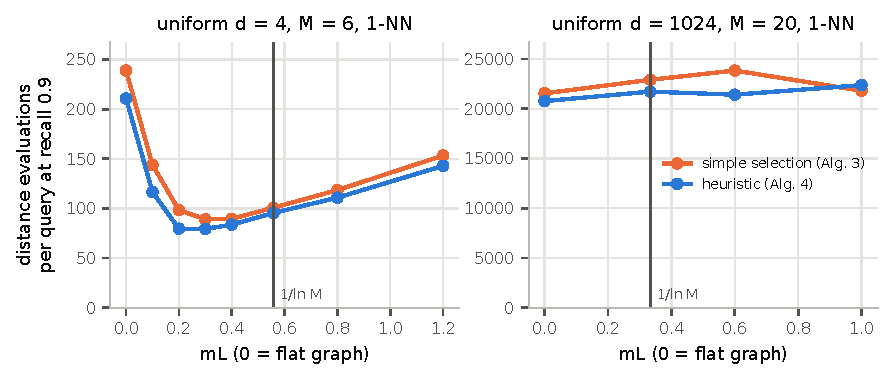
\includegraphics[width=0.98\linewidth]{hnsw_ml}
\caption{Cost of reaching recall 0.9 (1-NN) as a function of $m_L$, for the simple and the heuristic neighbour selection. The vertical line marks the paper's default $m_L=1/\ln M$.}
\label{fig:ml}
\end{figure}

\begin{figure}[t]
\centering
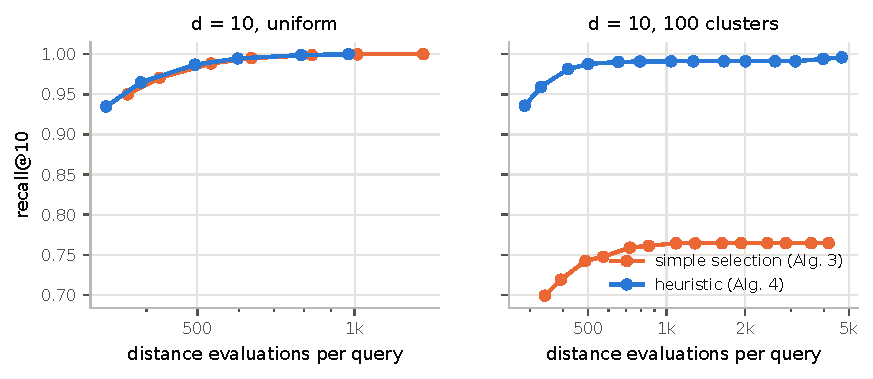
\includegraphics[width=0.98\linewidth]{hnsw_clusters}\\[0.3em]
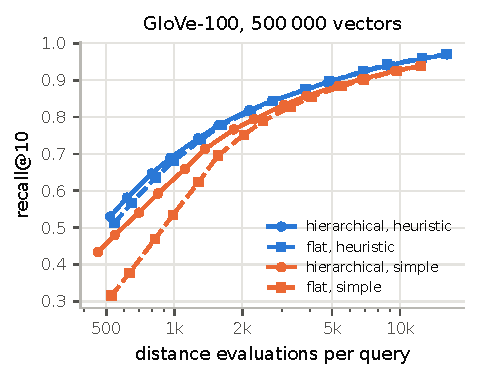
\includegraphics[width=0.49\linewidth]{hnsw_glove_flat}
\caption{Top: recall against cost on one million points in $d=10$, uniform and with 100 isolated clusters. Bottom: flat against hierarchical graphs on GloVe-100.}
\label{fig:clusters}
\end{figure}

\section{Folding the agent's score into the index}
\label{sec:fold}

\subsection{An exact inner-product form}

Leave the normalisation aside for a moment and consider the unnormalised score $a\,\rec_i+b\,\imp_i+c\,\rel_i$. Because the decay is exponential it factorises around any anchor time $\tau$,
\begin{equation}
\delta^{\,T-t_i} \;=\; \delta^{\,T-\tau}\;\delta^{\,\tau-t_i},
\end{equation}
where the first factor depends only on the query time and the second only on the memory. This is the idea behind forward decay in stream processing \citep{cormode2009forward}. For a construction scale $s>0$ define
\begin{equation}
x_i=\begin{bmatrix} e_i\\ s\,\delta^{\,\tau-t_i}\\ s\,\imp_i\end{bmatrix},\qquad
Q=\begin{bmatrix} c\,q\\ (a/s)\,\delta^{\,T-\tau}\\ b/s\end{bmatrix},\qquad
\langle Q,x_i\rangle \;=\; a\,\delta^{\,T-t_i}+b\,\imp_i+c\,\langle q,e_i\rangle .
\label{eq:fold}
\end{equation}
The identity holds for every memory, every query time and every choice of weights. Retrieving the best $k$ memories is therefore a maximum inner product search over $(d+2)$-dimensional vectors. HNSW can be built with the inner product as its similarity \citep{morozov2018ipnsw}. The memory vectors depend neither on the weights nor on the query time, so the same index serves an agent whose weights or clock change from one query to the next.

\citet{wei2026tango} have published the same identity, which they call score-preserving temporal reduction (STR), for a score made of similarity and an exponential decay of each item's creation time, and they build a dedicated graph index on top of it. This work arrived at the identity independently. Their setting has no importance term, no min-max normalisation and no timestamps that change after an item is inserted. These are exactly the parts an agent memory needs, and the rest of this section and \cref{sec:curves} deal with them.

\subsection{Min-max normalisation}

Min-max scaling subtracts the minimum of each component and divides by its range. For a given query the minima are constants that do not change the ranking. The ranges only rescale the weights:
\begin{equation}
\mathrm{score}_i=\frac{a}{R_{\rec}}\,\rec_i+\frac{b}{R_{\imp}}\,\imp_i+\frac{c}{R_{\rel}}\,\rel_i-\text{const}.
\end{equation}
The normalised top-$k$ is therefore the unnormalised top-$k$ with weights $(a/R_{\rec},\,b/R_{\imp},\,c/R_{\rel})$. Two of the ranges are cheap to maintain: $R_{\imp}$ from the smallest and largest importance and $R_{\rec}=\delta^{\,T-t_{\max}}-\delta^{\,T-t_{\min}}$ from the latest and earliest access times (a heap with lazy deletion tracks $t_{\min}$ while access times change). The relevance range depends on the query. Its maximum is the best match of $q$ and its minimum is the best match of $-q$, so two extra searches with $k=1$ on the same index estimate it.

\subsection{From a formula to a memory store}

Three practical problems remain.

\textbf{Bounded coordinates.} A memory accessed after the anchor has $\delta^{\,\tau-t_i}>1$, so the coordinate grows exponentially: by a factor of about 50\,000 over 90 days with $\delta=0.995$. Anchoring at the latest access time keeps every coordinate in $(0,1]$, but new memories keep arriving. The store therefore writes into a \emph{hot segment} anchored at its creation time and closes it after one week, so its coordinates stay below $\delta^{-168}\approx2.3$. When more than four closed segments exist, they are merged into a single index re-anchored at its latest access time, which also drops deleted entries. A query searches every segment, so it matters that their number stays bounded.

\textbf{Refresh on access.} Each retrieval resets the access time of the memories it returns, which changes their recency coordinate. The store marks them as deleted in their segment and moves them into a write buffer of 256 memories that is scored by a linear scan. A full buffer is flushed into the hot segment.

\textbf{Exact re-scoring.} The candidates from all segments and from the buffer are merged and scored with the exact formula. With LangChain's unnormalised score the approximation can therefore only miss memories, never reorder the ones it found. Under min-max scaling the candidates are ranked with the weights obtained from the estimated ranges, so they can also come out in a slightly different order from the exact score. \Cref{sec:static} shows that this is where most of the remaining loss comes from.

The inner product in \cref{eq:fold} is exact for any $s$, but the graph is built on the vectors $x_i$, so $s$ decides how much the two metadata coordinates shape the neighbourhoods. With a small $s$ the graph is essentially the semantic graph. With a large $s$ it groups memories by age and importance. \Cref{sec:static} measures the effect. The default is $s=1$.

\subsection{A retriever for LangChain}

\code{ExactTimeWeightedRetriever} scores documents like LangChain's retriever and keeps its main fields (decay rate, additional score keys such as importance, $k$, stamping of the access time), but keeps the documents in the folded store. It is not a complete drop-in replacement: it takes an embedding model instead of a vector store, has no asynchronous interface and reads the additional score keys when a document is added. LangChain does not normalise, so no range estimates are needed and the reduction is exact.

\section{Retrieval benchmark}
\label{sec:static}

\subsection{Setup}

\textbf{Data.} The scale test uses GloVe vectors (Twitter, 100 dimensions, unit length) as memory embeddings with synthetic agent metadata: creation times uniform over 90 days, 5\% of the memories accessed again later, importance drawn from the distribution observed in the town simulation of \cref{sec:town}. Metadata and embeddings are independent here, which is the least favourable case for similarity-based candidates. The second data set has realistic correlations: the pooled memory streams of the 25 Willowbrook agents after 92 simulated days (\TwN{} memories with simulated importance and access times) queried with the focal points the agents actually use.

\textbf{Methods.} \emph{Exact scan} scores every memory (NumPy, the ground truth). \emph{Relevance only} returns the $k$ most similar memories from an HNSW index, which is what a plain retrieval-augmented memory does. \emph{Overfetch and re-rank} fetches $K$ memories by similarity, adds the $k$ newest and re-ranks them with the full score, with the normalisation ranges estimated in the same way as for our store. \emph{Folded HNSW} is the store of \cref{sec:fold}. All HNSW indexes use hnswlib with $M=16$ and $ef_{\mathrm{construction}}=200$. Queries run on one thread and recall@10 is measured against the exact top-10 of the same score. The machine is a cloud virtual machine with two cores.

\subsection{Results}

\begin{figure}[t]
\centering
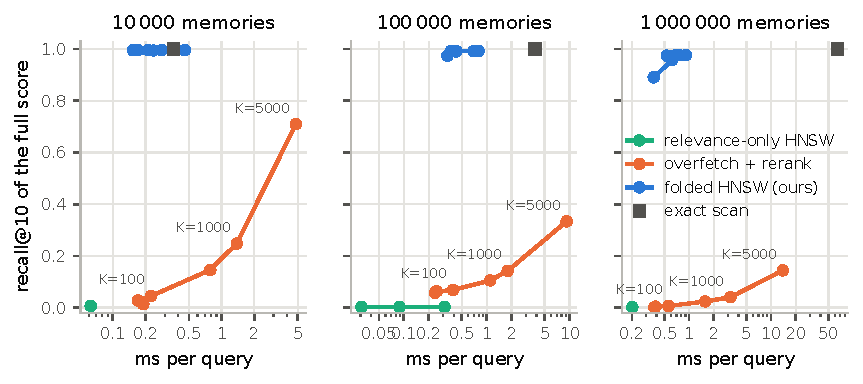
\includegraphics[width=0.99\linewidth]{static_tradeoff}
\caption{Recall@10 of the paper's score against query time on GloVe with synthetic metadata. Points along a curve are search depths ($ef$) or, for re-ranking, candidate counts $K$.}
\label{fig:tradeoff}
\end{figure}

\begin{figure}[t]
\centering
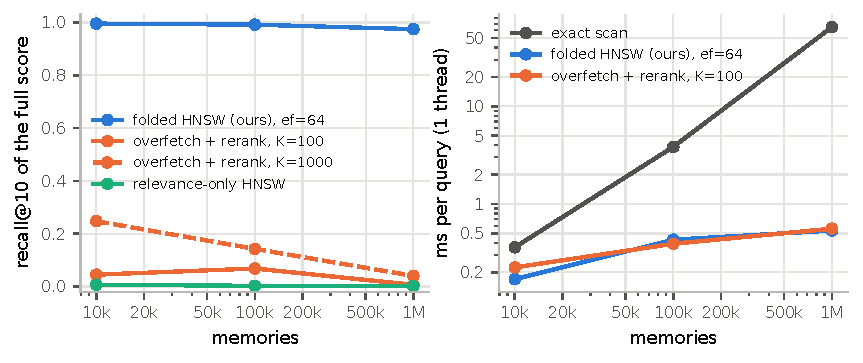
\includegraphics[width=0.99\linewidth]{static_scaling}
\caption{Recall (left) and query time (right) as the memory grows.}
\label{fig:scaling}
\end{figure}

\begin{table}[t]
\centering\small
\begin{tabular}{l ccc r ccc}
\toprule
 & \multicolumn{4}{c}{GloVe, 1\,000\,000 memories} & \multicolumn{3}{c}{Willowbrook, 126\,454 memories}\\
\cmidrule(lr){2-5}\cmidrule(lr){6-8}
Method & paper & code & raw & ms & paper & code & raw\\
\midrule
Exact scan & 1.000 & 1.000 & 1.000 & 64.5 & 1.000 & 1.000 & 1.000\\
Relevance only & 0.001 & 0.016 & 0.002 & 0.20 & 0.042 & 0.045 & 0.043\\
Overfetch + re-rank, $K=100$ & 0.006 & 0.083 & 0.010 & 0.56 & 0.277 & 0.325 & 0.290\\
Overfetch + re-rank, $K=1000$ & 0.040 & 0.298 & 0.059 & 3.18 & 0.661 & 0.769 & 0.729\\
Folded HNSW, $ef=64$ & 0.975 & 0.875 & 0.996 & 0.53 & 0.959 & 0.978 & 0.994\\
Folded HNSW, $ef=256$ & 0.976 & 0.959 & 1.000 & 0.69 & 0.962 & 0.981 & 0.999\\
\bottomrule
\end{tabular}

\caption{Recall@10 and query time with one million GloVe memories and on the pooled Willowbrook memories, for the three weight profiles: the paper's (min-max, $a=b=c=1$), the public code's weights (min-max, recency 0.5, importance 2, relevance 3) and LangChain's unnormalised sum. Folded HNSW and relevance only use $ef=64$.}
\label{tab:static}
\end{table}

\Cref{fig:tradeoff,fig:scaling,tab:static} summarise the benchmark. Three observations stand out.

\textbf{Similarity candidates miss most of the true top-$k$.} With the paper's weights, the 10 memories with the highest score are mostly recent and important ones, rarely among the most similar. Relevance-only retrieval recovers \GlRelonlyRecallOneM{} of them with one million memories and overfetch with $K=100$ recovers \GlRerankRecallOneM{}. More candidates help, but slowly: $K=1000$ reaches \GlRerankKRecallOneM{}. With $K=100$ it stays low at every size: \GlRerankRecallTenK{}, \GlRerankRecallHundredK{} and \GlRerankRecallOneM{} at 10\,000, 100\,000 and one million memories. On the town memories, where similarity and recency are correlated, the gap is smaller but still large (\TwRerankRecall{} for $K=100$).

\textbf{The folded index recovers almost all of the true top-$k$.} At $ef=64$ the folded store reaches \GlOursRecallOneM{} on one million memories and \TwOursRecall{} on the town memories. A deeper graph search hardly changes this (\GlOursRecallDeep{} at $ef=256$), because most of the remaining loss comes from the estimated relevance range. With the exact ranges, an $O(n)$ scan used here only for the analysis, the same index reaches \GlOursExactNorm{} and \TwOursExactNorm{}. The two range searches use a beam of 32 by default. \Cref{tab:normef}, from a separate build of the same indexes, shows that a wider beam closes most of the gap, at the price of a slower query: with a beam of 128, recall on one million memories rises from \NeGlA{} to \NeGlC{} and the query time from \NeGlMsA{} to \NeGlMsC{} ms.

With the weights of the public code, which put most of the weight on relevance (0.5 for recency, 2 for importance and 3 for relevance), the folded index needs a deeper search on GloVe: \GlCodeRecall{} at $ef=64$ and \GlCodeRecallDeep{} at $ef=256$. \Cref{sec:relsweep} explains why.

Index construction runs on two threads and is not deterministic, so two builds of the same index differ slightly. On the town memories, \BvBuilds{} builds (\code{experiments/exp\_buildvar.py} plus the builds behind \cref{tab:static,tab:normef}) gave recall between \BvPaperMin{} and \BvPaperMax{} at $ef=64$ with the paper's weights and between \BvCodeMin{} and \BvCodeMax{} with the code's weights. Differences of this size between the tables are noise.

\begin{table}[t]
\centering\small
\begin{tabular}{l rr rr}
\toprule
 & \multicolumn{2}{c}{GloVe, 1\,000\,000} & \multicolumn{2}{c}{Willowbrook, 126\,454}\\
\cmidrule(lr){2-3}\cmidrule(lr){4-5}
range search & recall@10 & ms & recall@10 & ms\\
\midrule
beam 32 (default) & 0.971 & 0.47 & 0.967 & 0.16\\
beam 64 & 0.982 & 0.57 & 0.970 & 0.17\\
beam 128 & 0.988 & 1.16 & 0.982 & 0.40\\
beam 256 & 0.991 & 1.70 & 0.984 & 0.38\\
exact ranges ($O(n)$ scan) & 0.997 & -- & 0.990 & --\\
\bottomrule
\end{tabular}

\caption{Recall@10 of the folded store ($ef=64$, paper's weights) and query time as the beam of the two searches that estimate the relevance range grows. The last row uses the exact range. The index is a separate build from the one in \cref{tab:static}.}
\label{tab:normef}
\end{table}

\textbf{It stays fast.} A linear scan of one million memories takes \GlExactMsOneM{} ms per query on one core when NumPy evaluates the full formula and about \GlExactMvMsOneM{} ms for the matrix-vector product alone, the least an exact scan can cost. The folded store answers in \GlOursMsOneM{} ms, \GlSpeedupMv{} to \GlSpeedupOneM{} times faster. Its query time grows slowly with the size of the memory (\cref{fig:scaling}).

\begin{figure}[t]
\centering
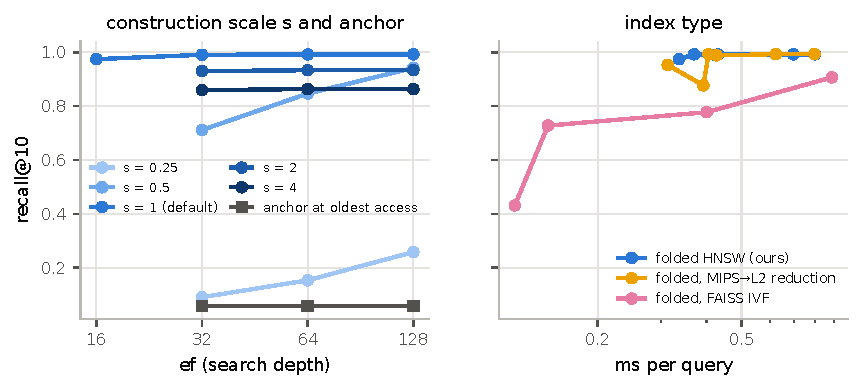
\includegraphics[width=0.99\linewidth]{static_ablation}
\caption{Ablations on 100\,000 GloVe memories with the paper's weights. Left: construction scale $s$ and the choice of anchor. Right: the same folded vectors in an inner-product HNSW index, in an HNSW index after the MIPS-to-Euclidean reduction and in a FAISS IVF-Flat index.}
\label{fig:ablation}
\end{figure}

\textbf{Ablations} (\cref{fig:ablation}). Anchoring at the oldest access time instead of the newest makes the recency coordinate span almost five orders of magnitude, so recall collapses to \AbOldAnchor{} whatever the search depth. The construction scale matters in both directions: $s=0.25$ hides the metadata from the graph (\AbSQuarter{} at $ef=128$), $s=4$ lets it dominate (\AbSFour{}) and $s=1$ gives \AbSOne{}. The classic reduction of MIPS to Euclidean search \citep{bachrach2014xbox} needs a deeper search than the inner-product graph for the same recall, which matches \citet{morozov2018ipnsw}. On the town memories it ends higher at large depths, though (\TwLtwoDeep{} against \TwIpDeep{} at $ef=512$), probably because its two range searches work better on a metric graph. The fold itself is not tied to HNSW. An IVF-Flat index from FAISS on the same vectors works too, with a worse trade-off on GloVe (\AbIvfRecall{} at \AbIvfMs{} ms with 64 probes, against \AbSOne{} at \AbOursMs{} ms for HNSW) and a better one on the town memories with the paper's weights (\TwIvfRecall{} at \TwIvfMs{} ms with 16 probes), though not with the code's weights (\TwIvfCodeRecall{}, against \TwOursCodeRecall{} for HNSW). With exact ranges HNSW reaches a similar \TwOursExactNorm{} on the paper's weights, which suggests that the advantage of IVF there comes from its range searches.

\subsection{When are similarity candidates enough?}
\label{sec:relsweep}

Overfetching is not always wrong. \Cref{tab:relsweep} raises the weight of relevance while keeping recency and importance at 1. Up to a relevance weight of 2 the folded index stays at or above \RsLowFoldedMin{} at $ef=64$, while overfetch never exceeds \RsLowRerankMax{}, even with $K=1000$. Between 4 and 8 the picture turns. Once relevance outweighs the other two terms several times over, the top-$k$ is mostly made of the most similar memories: at weight 8 overfetch with $K=1000$ reaches \RsEightRerankK{} and the folded index \RsEightFolded{} ($ef=64$) or \RsEightFoldedDeep{} ($ef=256$). At weight 16 even $K=100$ (\RsSixteenRerank{}) does better than the folded index at $ef=64$ (\RsSixteenFolded{}). The graph of the folded index was shaped partly by the metadata coordinates, so a query that ignores them needs a deeper search or a smaller construction scale. A store that serves both kinds of queries can route them by their weights, or use $s=0.5$, which stays above \RsHalfMin{} at $ef=256$ across the whole sweep.

\begin{table}[t]
\centering\small
\begin{tabular}{r ccc cccc}
\toprule
 & & \multicolumn{2}{c}{overfetch + re-rank} & \multicolumn{4}{c}{folded HNSW ($s$, $ef$)}\\
\cmidrule(lr){3-4}\cmidrule(lr){5-8}
relevance weight & rel.\ only & $K{=}100$ & $K{=}1000$ & $s{=}1$, 64 & $s{=}1$, 256 & $s{=}0.5$, 64 & $s{=}0.5$, 256\\
\midrule
0.25 & 0.001 & 0.096 & 0.123 & 0.996 & 0.996 & 0.768 & 0.985\\
0.5 & 0.001 & 0.081 & 0.118 & 0.994 & 0.994 & 0.816 & 0.985\\
1 & 0.002 & 0.068 & 0.142 & 0.992 & 0.993 & 0.849 & 0.983\\
2 & 0.018 & 0.093 & 0.245 & 0.983 & 0.988 & 0.848 & 0.978\\
4 & 0.105 & 0.336 & 0.660 & 0.909 & 0.969 & 0.854 & 0.970\\
8 & 0.366 & 0.699 & 0.954 & 0.759 & 0.909 & 0.835 & 0.956\\
16 & 0.634 & 0.848 & 0.983 & 0.695 & 0.868 & 0.814 & 0.938\\
32 & 0.746 & 0.858 & 0.970 & 0.706 & 0.854 & 0.805 & 0.924\\
\bottomrule
\end{tabular}

\caption{Recall@10 on 100\,000 GloVe memories as the relevance weight grows (recency and importance weights fixed at 1, min-max normalised).}
\label{tab:relsweep}
\end{table}

\subsection{LangChain}

The comparison with LangChain uses the real classes: the memory streams of five Willowbrook agents after 30 days (\LcMinN{}--\LcMaxN{} documents each), importance as an additional score key, cosine similarity as relevance, a decay rate of \LcDecay{} per hour so that recency matches the paper's 0.995 (LangChain's default is 0.01) and the agents' own planning and conversation focal points as queries. Measured against the exact top-10 of LangChain's own formula, LangChain's retriever returns \LcRecall{} of the right documents and our retriever returns \LcOursRecall{}.

\section{Agents in a town}
\label{sec:town}

\subsection{Willowbrook}

Willowbrook has twelve places (a café, a library, a college, a park, a pub, a town hall and others) and 25 residents with jobs, homes, weekly routines, favourite places and interests. Time advances in steps of 15 minutes. The cognitive loop follows Generative Agents, with every call to the language model replaced by a rule.
\begin{itemize}
\item \textbf{Perception.} At every step a resident observes what it is doing and what up to three other people at the same place are doing. New observations enter its memory stream with an importance that depends on the activity (sleeping 1, routine at home 2, work or leisure 3, chatting 4, attending an event 7) plus a small random offset.
\item \textbf{Conversation.} Residents at the same place talk with a probability that depends on their sociability. Before talking, the speaker retrieves memories with the focal points used by \code{converse.py} in the reference code, the listener's name ($k=50$) and ``\emph{listener} is \emph{activity}'' ($k=25$). With probability 0.5 it then passes on the most important piece of news among the retrieved memories that it has not yet exchanged with this listener, otherwise the two make small talk. Both remember the conversation.
\item \textbf{Planning.} At wake-up and at 14:00 every resident retrieves memories with the focal points of \code{plan.py}, ``\emph{name}'s plan for \emph{date}.'' and ``Important recent events for \emph{name}'s life.'' ($k=30$ each). If an event of that day is among the retrieved memories, the resident attends it with a fixed probability.
\item \textbf{News.} Every eight hours somebody learns a piece of gossip (a new puppy, a promotion, a picnic on Thursday). The scenario of the paper is reproduced on top of this: Maria Lopez, who runs the café, learns 35 hours in advance that she is hosting a party there at 5 pm. She invites everyone she talks to.
\end{itemize}
Every retrieval refreshes the access time of the memories it returns. Random decisions use counter-based hashing, so two runs with the same seed see the same world and diverge only where their retrievals differ.

\textbf{Calibration.} Two parameters have no counterpart in the paper, the conversation rate and the probability of passing on news. They were chosen with exact retrieval in a young town (two days of memories) so that the outcome matches the Valentine's Day party of \citet{park2023generative}, where 13 of the 25 agents knew about the party after two game days and 5 of the 12 invited agents came. Over a grid of 15 settings with 12 seeds each (\code{experiments/calibrate\_town.py}), a conversation rate of 0.06 and a sharing probability of 0.5 give \CalKnew{} knowing agents and \CalAttended{} guests on average.

\textbf{Experiment.} The independent variable is the age of the town when Maria learns about the party: 2 days, as in the paper, or 9, 32 or 92 days, so that every agent carries a larger memory into the scenario. Each age was run with 30 seeds and four retrieval methods, all with the paper's score (min-max, $a=b=c=1$): the exact scan, the folded store, overfetch with $K=100$ and relevance only. The outcomes are the number of agents who knew about the party before it started, who had it among their retrieved memories when planning the day and who attended.

\subsection{Results}

\Cref{fig:town,tab:town} show the outcomes. In a young town the four methods agree: with about a hundred memories per agent, the party ranks high under any of them. From nine days on they drift apart, because the approximate methods return a shrinking share of the paper's top-$k$ as the memories grow: after three months, \TNinetyReRecall{} for overfetch and \TNinetyRelRecall{} for relevance only (\cref{fig:garecency}, right).

\textbf{The folded store behaves like the exact scan.} Its retrievals contain \TNinetyFoRecall{} of the paper's top-$k$ after 92 days. The three outcomes are identical on every seed up to 32 days and on \TNinetyFoSame{} of the \TNinetySeeds{} seeds at 92 days. On the other seeds they differ by at most \TNinetyFoMaxDiff{} agents, in both directions.

\textbf{Relevance-only memory loses about 40\% of the diffusion.} From nine days on, \TRelDropAwareLo{} to \TRelDropAwareHi{} fewer agents know about the party and \TRelDropAttLo{} to \TRelDropAttHi{} fewer attend it (\TNinetyRelAware{} against \TNinetyExAware{} knowing agents and \TNinetyRelAtt{} against \TNinetyExAtt{} guests at 92 days). The invitation travels through conversations. The focal point of a conversation is the listener's name, which the party is rarely similar to. Without recency and importance the agents do not think of mentioning it.

\textbf{Overfetch and re-rank moves the outcome in both directions.} At 9 and 32 days it spreads the news slightly less than the exact scan (\TThirtyReAware{} against \TThirtyExAware{} knowing agents at 32 days). At 92 days it spreads it clearly more: \TNinetyReAware{} agents know about the party and \TNinetyReRecalled{} recall it when planning, against \TNinetyExAware{} and \TNinetyExRecalled{}, although it returns less than half of the paper's top-$k$. The reason is the second half of its candidate set, the newest memories. A piece of news is among an agent's newest memories right after it is heard, so it always becomes a candidate, while most of the recent observations that would outrank it under the full score are neither that new nor similar enough to the focal point and never reach the re-ranking. Taking the newest memories out of the candidate set confirms this. With only the 100 most similar memories, the outcome at 92 days falls to \TNinetyNrAware{} knowing agents and \TNinetyNrAtt{} guests (\TThirtyNrAware{} and \TThirtyNrAtt{} at 32 days), close to relevance-only memory, although the share of the paper's top-$k$ it retrieves hardly changes (\TNinetyNrRecall{} against \TNinetyReRecall{}).

Two conclusions follow. An approximate retrieval does not lose information at random: it changes which information the agents act on. The direction of the change depends on details such as which recent memories enter the candidate set and how large the memory has grown. And recall against the paper's top-$k$ does not predict the effect, since two methods with the same recall led the town to very different outcomes.

\begin{figure}[t]
\centering
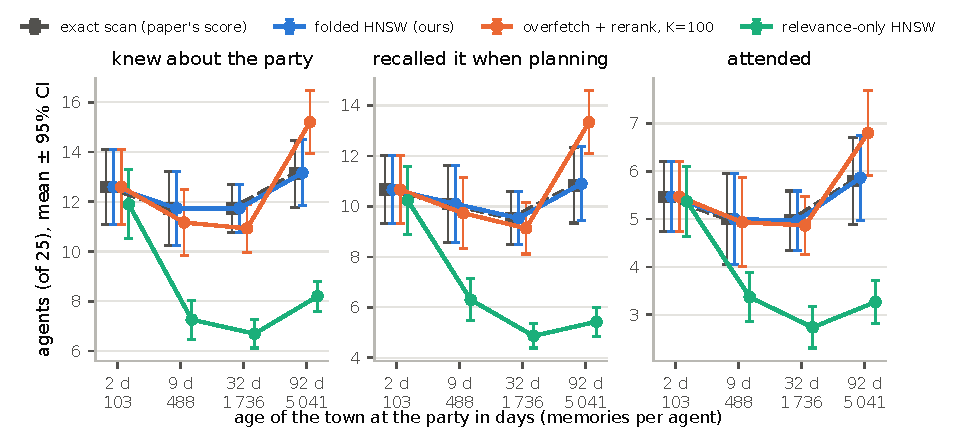
\includegraphics[width=0.99\linewidth]{town_outcomes}
\caption{The party scenario in towns of increasing age (30 seeds each, mean and 95\% confidence interval). The folded store reproduces the exact scan on every seed up to 32 days and on \TNinetyFoSame{} of \TNinetySeeds{} at 92 days.}
\label{fig:town}
\end{figure}

\begin{table}[t]
\centering\small
\begin{tabular}{l l r r r r r}
\toprule
Age & Retrieval & memories & recall & knew & recalled & attended\\
\midrule
2 days & Exact scan (paper) & 103 & 1.000 & 12.6 $\pm$ 1.5 & 10.7 $\pm$ 1.3 & 5.5 $\pm$ 0.7\\
 & Folded HNSW (ours) & 103 & 1.000 & 12.6 $\pm$ 1.5 & 10.7 $\pm$ 1.3 & 5.5 $\pm$ 0.7\\
 & Overfetch + re-rank, $K{=}100$ & 103 & 0.995 & 12.6 $\pm$ 1.5 & 10.7 $\pm$ 1.3 & 5.5 $\pm$ 0.7\\
 & Relevance only & 103 & 0.872 & 11.9 $\pm$ 1.4$^{**}$ & 10.2 $\pm$ 1.3$^{**}$ & 5.4 $\pm$ 0.7\\
\addlinespace
9 days & Exact scan (paper) & 488 & 1.000 & 11.7 $\pm$ 1.5 & 10.1 $\pm$ 1.5 & 5.0 $\pm$ 1.0\\
 & Folded HNSW (ours) & 488 & 1.000 & 11.7 $\pm$ 1.5 & 10.1 $\pm$ 1.5 & 5.0 $\pm$ 1.0\\
 & Overfetch + re-rank, $K{=}100$ & 487 & 0.876 & 11.2 $\pm$ 1.3$^{**}$ & 9.7 $\pm$ 1.4$^{*}$ & 4.9 $\pm$ 0.9\\
 & Relevance only & 484 & 0.637 & 7.3 $\pm$ 0.8$^{**}$ & 6.3 $\pm$ 0.8$^{**}$ & 3.4 $\pm$ 0.5$^{**}$\\
\addlinespace
32 days & Exact scan (paper) & 1736 & 1.000 & 11.7 $\pm$ 1.0 & 9.5 $\pm$ 1.0 & 5.0 $\pm$ 0.6\\
 & Folded HNSW (ours) & 1736 & 1.000 & 11.7 $\pm$ 1.0 & 9.5 $\pm$ 1.0 & 5.0 $\pm$ 0.6\\
 & Overfetch + re-rank, $K{=}100$ & 1734 & 0.681 & 10.9 $\pm$ 1.0$^{*}$ & 9.1 $\pm$ 1.0$^{*}$ & 4.9 $\pm$ 0.6\\
 & Relevance only & 1725 & 0.488 & 6.7 $\pm$ 0.6$^{**}$ & 4.9 $\pm$ 0.5$^{**}$ & 2.7 $\pm$ 0.4$^{**}$\\
\addlinespace
92 days & Exact scan (paper) & 5041 & 1.000 & 13.1 $\pm$ 1.3 & 10.8 $\pm$ 1.5 & 5.8 $\pm$ 0.9\\
 & Folded HNSW (ours) & 5041 & 0.999 & 13.2 $\pm$ 1.3 & 10.9 $\pm$ 1.5 & 5.9 $\pm$ 0.9\\
 & Overfetch + re-rank, $K{=}100$ & 5034 & 0.487 & 15.2 $\pm$ 1.3$^{**}$ & 13.3 $\pm$ 1.3$^{**}$ & 6.8 $\pm$ 0.9$^{*}$\\
 & Relevance only & 5007 & 0.366 & 8.2 $\pm$ 0.6$^{**}$ & 5.4 $\pm$ 0.6$^{**}$ & 3.3 $\pm$ 0.5$^{**}$\\
\bottomrule
\end{tabular}

\caption{The party scenario by age of the town. Memories per agent at the end of the run, mean recall of the paper's top-$k$ over all retrievals and the number of agents (of 25) who knew about the party, recalled it when planning and attended, as mean $\pm$ 95\% confidence interval over 30 seeds. Stars mark a difference from the exact scan in a paired Wilcoxon test ($^{*}p<0.05$, $^{**}p<0.01$).}
\label{tab:town}
\end{table}


\section{Beyond exponential recency}
\label{sec:curves}

% Section: forgetting curves beyond the exponential (input from main.tex)

\subsection{Why another curve}

The paper's recency term looks only at the last access and halves every 138 hours. Memory research describes forgetting differently. \citet{anderson1991reflections} measured how often an item comes back in natural environments (newspaper headlines, speech to children, electronic mail) and found that the probability of needing it again falls as a power of the time since each earlier occurrence and grows with the number of occurrences. Human retention follows the same power law \citep{wixted1991form}. ACT-R turns this into the base-level activation of a memory, $B_i=\ln\sum_j (T-t_{ij})^{-d}$ with $d=0.5$, a sum over every past use \citep{anderson2004integrated}. Agent memories have started to borrow such curves. MemoryBank strengthens a memory each time it is recalled \citep{zhong2024memorybank} and FadeMem decays memories with a stretched exponential \citep{wei2026fademem}. These systems say little about how to search a large memory under such a score, and the time-decayed vector search of \citet{wei2026tango} handles a single exponential of a fixed creation time.

This section uses the score
\begin{equation}
\mathrm{score}_i = a\,\widehat{D}_i + b\,\widehat{\imp}_i + c\,\widehat{\rel}_i,\qquad
D_i(T)=\sum_j \varphi(T-t_{ij}),\qquad \varphi(\Delta)=\Bigl(1+\frac{\Delta}{h_0}\Bigr)^{-d},
\label{eq:curvescore}
\end{equation}
where $t_{i1}<t_{i2}<\dots$ are the times at which memory $i$ was created or retrieved, $d=0.5$ as in ACT-R and $h_0=1$ hour keeps the curve finite at age zero. The hats are min-max scaling as before and $a=b=c=1$. This is ACT-R's sum without the logarithm, which cannot be folded (\cref{sec:curvelimits}). A second variant keeps only the last use, $D_i=\varphi(T-t_i)$, so that the curve is the only change from the paper.

\subsection{Any such curve is an inner product}

The power law, the hyperbolic curve $1/(1+\Delta/h)$ and stretched exponentials $e^{-\lambda\Delta^\beta}$ with $\beta\le1$ are completely monotone. By Bernstein's theorem every such function is a mixture of exponentials, $\varphi(\Delta)=\int e^{-\lambda\Delta}\,d\mu(\lambda)$ with $\mu\ge0$ \citep{widder1941laplace}, and a few terms of the mixture approximate it closely over any bounded range of ages \citep{beylkin2005expsums}:
\begin{equation}
\varphi(\Delta)\;\approx\;\varphi_R(\Delta)=\sum_{r=1}^{R} w_r\,e^{-\lambda_r\Delta},\qquad w_r\ge0 .
\end{equation}
The rates are spaced geometrically and the weights are fitted by non-negative least squares, with every error divided by the value of the curve, floored at 1\% of its start (\code{agentmem/curves.py}). \Cref{tab:curvefit} shows that the error shrinks quickly with $R$: eight exponentials follow ACT-R's curve over a whole year with an error of at most \CfActrRngEight{} of its range.

\begin{table}[t]
\centering\small
\begin{tabular}{r rr rr rr}
\toprule
 & \multicolumn{2}{c}{ACT-R} & \multicolumn{2}{c}{hyperbolic} & \multicolumn{2}{c}{FadeMem}\\
\cmidrule(lr){2-3}\cmidrule(lr){4-5}\cmidrule(lr){6-7}
$R$ & of range & relative & of range & relative & of range & relative\\
\midrule
4 & 5.82\% & 10.65\% & 3.00\% & 6.83\% & 2.76\% & 6.86\%\\
6 & 2.58\% & 3.47\% & 0.47\% & 1.01\% & 1.23\% & 2.24\%\\
8 & 0.30\% & 0.59\% & 0.06\% & 0.16\% & 0.36\% & 0.65\%\\
10 & 0.10\% & 0.14\% & 0.01\% & 0.03\% & 0.59\% & 0.62\%\\
12 & 0.02\% & 0.04\% & 0.00\% & 0.01\% & 0.20\% & 0.27\%\\
\bottomrule
\end{tabular}

\caption{Largest error of a sum of $R$ exponentials over ages from 0 to one year, as a share of the curve's range and relative to the curve where it is above 1\% of its start. ACT-R: $(1+\Delta/1\,\mathrm{h})^{-0.5}$. Hyperbolic: $1/(1+\Delta/24\,\mathrm{h})$. FadeMem: $e^{-0.1\,t^{0.8}}$ with $t$ in days, the long-term setting of \citet{wei2026fademem}.}
\label{tab:curvefit}
\end{table}

Every term of $\varphi_R$ factorises around an anchor $\tau$ as in \cref{eq:fold}, so
\begin{equation}
D^R_i(T)=\sum_{r=1}^{R} e^{-\lambda_r(T-\tau)}\;w_r\sum_j e^{-\lambda_r(\tau-t_{ij})}=\langle g(T),\,z_i(\tau)\rangle ,
\end{equation}
and with $x_i=[\,e_i;\ s\,z_i;\ s\,\imp_i\,]$ and $Q=[\,c\,q;\ (a/s)\,g(T);\ b/s\,]$ the score with the fitted curve is again $\langle Q,x_i\rangle$, now over $d+R+1$ dimensions. A memory does not need its whole history. It keeps $y_{ir}=\sum_j e^{-\lambda_r(t_i-t_{ij})}$ and its last use $t_i$, from which $z_{ir}(\tau)=w_r\,y_{ir}\,e^{-\lambda_r(\tau-t_i)}$, and a new use at time $t$ updates $y_{ir}\leftarrow y_{ir}\,e^{-\lambda_r(t-t_i)}+1$ in $O(R)$. Frequency therefore costs nothing extra. The paper's score is the case $R=1$ with $y_i\equiv1$.

The fit and the index are separate approximations. If $|\varphi_R-\varphi|\le\varepsilon\,\varphi$ on the ages that occur, then $|D^R_i-D_i|\le\varepsilon D_i$ for every memory, and when the fitted score of every memory is within $\eta$ of its true score, every memory in the fitted top-$k$ has a true score within $2\eta$ of the true $k$-th best. In the benchmark below an exact scan with the fitted curve returns \CuFitRecallOneM{} of the true top-10.

\subsection{A store for any curve}

The fitted rates span several orders of magnitude: for ACT-R's curve with $R=8$ the fastest is \CfFastRate{} per hour. The coordinate $e^{-\lambda_r(\tau-t_i)}$ of a memory used after the anchor grows by that factor every hour, so the hot segment of \cref{sec:fold}, anchored when it opens and filled for a week, no longer works. The store for general curves (\code{CurveFolded} in \code{agentmem/curve\_stores.py}) changes the order of events instead.
\begin{itemize}
\item A memory stays in a \emph{recent part} while its last use is younger than $W$ hours. The recent part is scored by a linear scan.
\item After that it moves to the hot segment. A hot segment is open for $L\le W$ hours and is anchored at $\tau=T_{\mathrm{open}}+L-W$.
\item Closed segments are merged as before and re-anchored at their latest use.
\end{itemize}
A memory enters a segment only when $t_i<T-W\le\tau$, so every stored coordinate lies in $[0,\,w_r\,y_{ir}]$ and every query factor $e^{-\lambda_r(T-\tau)}$ in $(0,1]$, for every rate, however fast. A retrieval moves the memories it returns back to the recent part, as the write buffer did before. The defaults are $W=L=24$ hours.

The normalisation needs the range of $D$. For a query factor with positive entries, $\max_i\langle g,z_i\rangle$ is reached on the Pareto-maximal set of the stored $z_i$ (those not dominated in every coordinate by another) and the minimum on the Pareto-minimal set, so the range of $D$ needs no search. The fronts are small: of the \CuSegN{} memories in the largest segment of the 100\,000-memory benchmark, \CuFrontMax{} are Pareto-maximal and \CuFrontMin{} Pareto-minimal. Deleting a memory that is not on a front leaves the fronts unchanged. The relevance range is estimated with the two searches for $\pm q$ as before, and small segments are simply scanned.

\subsection{Results}

\textbf{Retrieval at scale.} The benchmark of \cref{sec:static} is repeated with the score of \cref{eq:curvescore}. Every memory gets a use history: it is created at a uniform time over 90 days and used again a geometric number of times (1.2 on average) at uniform times after its creation. \Cref{tab:curvesstatic,fig:curves} show the results. An exact scan with the fitted curve returns \CuFitRecallOneM{} of the true top-10 with one million memories, so the fit itself costs almost nothing. The folded store returns \CuOursRecallHundredK{} of it with 100\,000 memories in \CuOursMsHundredK{} ms and \CuOursRecallOneM{} with one million in \CuOursMsOneM{} ms ($ef=64$). Overfetch returns \CuRerankOneM{} with $K=100$ and \CuRerankKOneM{} with $K=1000$, although it is given the exact normalisation ranges. Relevance only returns \CuRelOneM{}.

With one million memories most of the query time goes into the scan of the recent part, which in this history holds the \CuRecentOneM{} memories used in the last 24 hours. A recent part of 6 hours holds \CuRecentSixOneM{} memories and answers in \CuOursSixMsOneM{} ms, with recall \CuOursSixRecallOneM{}. More exponentials help up to a point: on 100\,000 memories at $ef=128$ recall is \CuRFour{}, \CuRSix{}, \CuREight{} and \CuRTen{} for $R=4$, 6, 8 and 10. As with the paper's score, part of the remaining loss comes from the estimated relevance range: with exact ranges the store reaches \CuRangeExact{} instead of \CuRangeEst{} on 100\,000 memories. The exact scan in this code takes \CuFitMsOneM{} ms per query on one million memories because it evaluates eight exponentials for every memory. Even a bare matrix-vector product, the least an exact scan can cost, takes about \GlExactMvMsOneM{} ms (\cref{sec:static}).

The curve changes what is retrieved. On the same one million memories, only \CuOverlapOneM{} of the top-10 under the ACT-R score are also in the top-10 under the paper's score (\CuOverlapHundredK{} with 100\,000 memories). Which curve suits an agent is a modelling question that this report does not answer. The point is that the index no longer constrains the answer.

\begin{table}[t]
\centering\small
\begin{tabular}{l rr rr}
\toprule
 & \multicolumn{2}{c}{100\,000 memories} & \multicolumn{2}{c}{1\,000\,000 memories}\\
\cmidrule(lr){2-3}\cmidrule(lr){4-5}
Method & recall@10 & ms & recall@10 & ms\\
\midrule
Exact scan, fitted curve ($R{=}8$) & 0.999 & 17 & 0.996 & 268\\
Folded HNSW, $ef{=}64$ (ours) & 0.982 & 0.70 & 0.969 & 2.40\\
Folded HNSW, $ef{=}256$ (ours) & 0.989 & 1.05 & 0.975 & 2.87\\
Folded HNSW, $ef{=}64$, $W{=}6$\,h (ours) & -- & -- & 0.954 & 1.55\\
Overfetch + re-rank, $K{=}100$ & 0.085 & 0.57 & 0.030 & 0.48\\
Overfetch + re-rank, $K{=}1000$ & 0.438 & 2.05 & 0.101 & 2.77\\
Relevance only & 0.014 & -- & 0.008 & --\\
\bottomrule
\end{tabular}

\caption{Recall@10 under the ACT-R score of \cref{eq:curvescore} (min-max, $a=b=c=1$, every use counted) on GloVe memories with synthetic use histories, and median query time. The folded store uses $R=8$ and a recent part of $W=24$ hours unless stated. Overfetch is given the exact normalisation ranges.}
\label{tab:curvesstatic}
\end{table}

\begin{figure}[t]
\centering
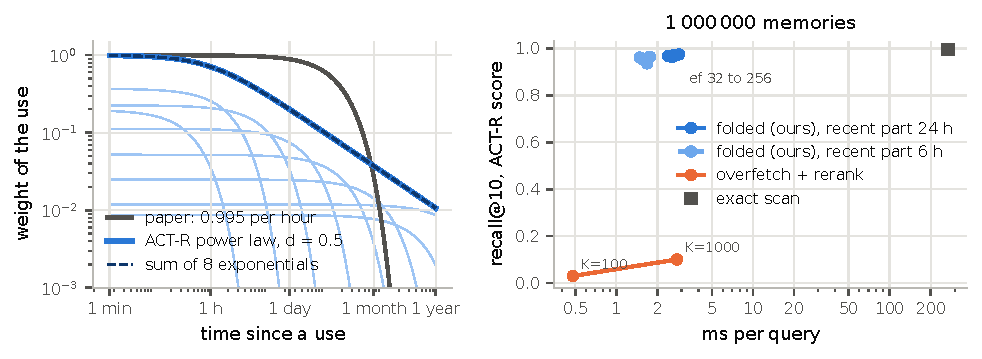
\includegraphics[width=0.99\linewidth]{curves}
\caption{Left: the weight of one use as a function of its age, for the paper's exponential and ACT-R's power law, with the eight exponentials (thin lines) whose sum (dashed) follows the power law. Right: recall@10 under the ACT-R score against query time with one million memories. Points along the folded curves are search depths, along overfetch candidate counts.}
\label{fig:curves}
\end{figure}

\subsection{Agents with a forgetting curve}
\label{sec:curvestown}

The party scenario of \cref{sec:town} was run again in the 32-day and 92-day runs, on the same 30 seeds, with ACT-R's curve in place of the paper's recency term. The curve takes two forms, of the last use only and summed over every use (\cref{eq:curvescore}). Each form is retrieved by an exact scan with the true curve, by the folded store ($R=8$, $W=L=24$ hours) and by overfetch and re-rank ($K=100$, with the newest memories added as in LangChain and exact normalisation ranges). In the town every segment is small enough for the folded store to compute its ranges by a scan. A third form takes ACT-R's logarithm of the sum. It cannot be folded and was run with the exact scan only. Recall is measured at every retrieval against the exact scan of the same score. \Cref{tab:curvestown} shows the outcomes.

\textbf{The folded store behaves like the exact scan with both foldable forms.} In the 92-day runs its retrievals contain \TcNinetyLastFoRecallFour{} of the true top-$k$ with the last use and \TcNinetyUsesFoRecallFour{} with every use. The three outcomes are identical on \TcNinetyLastFoSame{} and \TcNinetyUsesFoSame{} of the 30 seeds and differ by at most \TcNinetyUsesFoMaxDiff{} agents on the others. In the 32-day runs they are identical on \TcThirtyLastFoSame{} and \TcThirtyUsesFoSame{} seeds, with a largest difference of \TcThirtyUsesFoMaxDiff{} agents. At this memory size the exact scan is faster (\TcNinetyExMs{} against \TcNinetyFoMs{} ms per retrieval), as with the paper's score.

\textbf{The curve itself changes what the town does.} With exact retrieval and ACT-R's curve of the last use, \TcNinetyLastExAware{} agents know about the party at 92 days and \TcNinetyLastExRecalled{} recall it when planning, against \TcNinetyExpAware{} and \TcNinetyExpRecalled{} under the paper's exponential on the same seeds (paired Wilcoxon, Holm-adjusted $p=\TcNinetyLastVsExpAwareHolm{}$ and $p=\TcNinetyLastVsExpRecalledHolm{}$). In the 32-day runs the two curves give similar outcomes. The power law falls steeply in the first hours and slowly after that. After min-max scaling over 92 days, a memory last used five hours earlier keeps \TcShapeActrFive{} of the recency range under ACT-R's curve and \TcShapeExpFive{} under the exponential, one used 35 hours earlier \TcShapeActrThirtyFive{} and \TcShapeExpThirtyFive{}. Recency then mostly separates the last few hours from everything else, and among older memories importance weighs more. This probably helps the invitation, which is more important than most of what an agent observes.

\textbf{Counting every use locks the memory in.} With the sum over every use, only \TcNinetyUsesExRecalled{} agents recall the party when planning at 92 days and \TcNinetyUsesExAtt{} attend it, against \TcNinetyLastExRecalled{} and \TcNinetyLastExAtt{} with the last use (\TcThirtyUsesExRecalled{} against \TcThirtyLastExRecalled{} recalling it at 32 days). Every memory a retrieval returns counts as a use, so a memory that is retrieved gains weight and is retrieved again. Retrieval is concentrated under every form of the curve. At the end of \TcDiagSeeds{} of the 92-day runs, the 1\% most retrieved memories of an agent had received \TcDiagLastTopShare{} of its retrievals with the last use and \TcDiagUsesTopShare{} with every use. They are mostly pieces of news heard from other residents, which conversations bring up again and again. What differs is the effect on the score. With the last use a memory's recency term cannot exceed that of a fresh memory, so a memory heard an hour earlier still gets \TcDiagLastNewHour{} of the normalised range. Summed over every use, the most retrieved memories reach values of $D$ far above any single use, and the same memory gets \TcDiagUsesNewHour{}. ACT-R's logarithm compresses the range (\TcDiagLogNewHour{}) but changes the outcome little. With it the exact scan gives \TcNinetyLogExAware{} knowing agents, \TcNinetyLogExRecalled{} recalling the party and \TcNinetyLogExAtt{} guests. The lock-in therefore comes from counting retrievals as uses, not from leaving out the logarithm.

\textbf{Overfetch hides the problem.} With every use counted, overfetch returns only \TcNinetyUsesReRecall{} of the true top-$k$ at 92 days, yet \TcNinetyUsesReAware{} agents know about the party. Most of the memories that lock the score in probably never enter its candidate set, while the newest memories always do. Its outcome resembles the score of the last use more than the score it is meant to compute.

The index therefore no longer restricts the choice of curve, but the choice has to be tested in a closed loop. A score that looks reasonable on its own can lock an agent's memory in once every retrieval counts as a use.

\begin{table}[t]
\centering\small
\setlength{\tabcolsep}{4.5pt}
\begin{tabular}{l l l r r r r r}
\toprule
Run & Curve & Retrieval & memories & recall & knew & recalled & attended\\
\midrule
32 days & last use & Exact scan & 1736 & 1.000 & 12.1 $\pm$ 1.0 & 9.8 $\pm$ 1.1 & 5.1 $\pm$ 0.7\\
 &  & Folded HNSW (ours) & 1736 & 1.000 & 12.1 $\pm$ 1.0 & 9.8 $\pm$ 1.1 & 5.1 $\pm$ 0.7\\
 &  & Overfetch, $K{=}100$ & 1733 & 0.703 & 10.9 $\pm$ 1.0$^{**}$ & 9.1 $\pm$ 1.1$^{*}$ & 4.9 $\pm$ 0.6\\
\addlinespace[2pt]
 & every use & Exact scan & 1735 & 1.000 & 9.5 $\pm$ 1.0 & 5.8 $\pm$ 1.1 & 3.3 $\pm$ 0.6\\
 &  & Folded HNSW (ours) & 1735 & 1.000 & 9.3 $\pm$ 1.0 & 5.6 $\pm$ 1.0 & 3.2 $\pm$ 0.5\\
 &  & Overfetch, $K{=}100$ & 1734 & 0.601 & 10.9 $\pm$ 1.0$^{*}$ & 9.0 $\pm$ 1.1$^{**}$ & 4.8 $\pm$ 0.6$^{**}$\\
\addlinespace[2pt]
 & every use, log & Exact scan & 1736 & 1.000 & 10.0 $\pm$ 1.0 & 7.1 $\pm$ 1.0 & 3.9 $\pm$ 0.6\\
\addlinespace
92 days & last use & Exact scan & 5041 & 1.000 & 15.2 $\pm$ 1.4 & 12.4 $\pm$ 1.7 & 6.5 $\pm$ 1.0\\
 &  & Folded HNSW (ours) & 5041 & 1.000 & 15.1 $\pm$ 1.4 & 12.3 $\pm$ 1.7 & 6.4 $\pm$ 1.0\\
 &  & Overfetch, $K{=}100$ & 5033 & 0.536 & 15.2 $\pm$ 1.3 & 13.3 $\pm$ 1.3 & 6.8 $\pm$ 0.9\\
\addlinespace[2pt]
 & every use & Exact scan & 5034 & 1.000 & 9.2 $\pm$ 0.8 & 1.4 $\pm$ 0.2 & 1.2 $\pm$ 0.2\\
 &  & Folded HNSW (ours) & 5034 & 1.000 & 9.1 $\pm$ 0.8 & 1.4 $\pm$ 0.2 & 1.2 $\pm$ 0.2\\
 &  & Overfetch, $K{=}100$ & 5032 & 0.456 & 15.2 $\pm$ 1.3$^{**}$ & 11.5 $\pm$ 1.4$^{**}$ & 5.9 $\pm$ 0.9$^{**}$\\
\addlinespace[2pt]
 & every use, log & Exact scan & 5034 & 1.000 & 9.8 $\pm$ 1.0 & 2.8 $\pm$ 0.5 & 1.8 $\pm$ 0.3\\
\bottomrule
\end{tabular}

\caption{The party scenario with ACT-R's curve in place of the paper's recency term, of the last use, summed over every use and, with the exact scan only, the logarithm of that sum. Columns as in \cref{tab:town}. Recall is against the exact scan of the same score. Stars mark a difference from that exact scan in a paired Wilcoxon test, Holm-corrected over the 24 comparisons in the table ($^{*}p<0.05$, $^{**}p<0.01$).}
\label{tab:curvestown}
\end{table}

\subsection{Limits}
\label{sec:curvelimits}

\begin{itemize}
\item ACT-R takes the logarithm of the sum before adding other sources of activation. The logarithm does not change which of two memories has the larger recency-frequency term, but it changes how that term trades off against importance and relevance, and the logarithm of an inner product is not an inner product. The score used here keeps the sum, which favours frequently used memories more than ACT-R does. In the town the logarithm changes little (\cref{sec:curvestown}).
\item What locks the memory in is that every retrieved memory counts as a use. Remedies that still fold exist, for example a smaller weight for a retrieval than for the observation itself or a cap on the number of uses that count, but they are not tested here.
\item The curve's parameters are ACT-R's usual choices, not values fitted to agents, and the use histories of the scale test are synthetic.
\item Decay rates that differ from memory to memory, as in MemoryBank and FadeMem, fold only when they take a few values, with one block of coordinates per value. This is not implemented.
\item The recent part is scanned, so its cost grows with the number of memories used in the last $W$ hours. Compaction rebuilds the merged segment from scratch, which is cheap for one agent's memory but would need a tiered scheme for millions of memories.
\end{itemize}


\section{The reference implementation}
\label{sec:reference}

In the public code of Generative Agents \citep{ga_code}, retrieval is the function \code{new\_retrieve} of \code{retrieve.py}. Running that function unmodified on mock personas, with only the OpenAI embedding call replaced, shows three differences from Section 4.1 of the paper.
\begin{enumerate}
\item Recency depends on rank, not on time: the memories are sorted by access time and the $j$-th one receives $\delta^{\,j}$, whatever the number of hours between them ($\delta=0.995$ for the 25 agents of the paper's main scenario, 0.99 by default).
\item The sort is ascending, so the memory accessed longest ago comes first and receives the highest recency. The memory accessed most recently receives the lowest. After min-max scaling these become 1 and 0 (\cref{fig:garecency}).
\item The weights are $0.5$ for recency, $3$ for relevance and $2$ for importance instead of all ones.
\end{enumerate}
The heavier relevance weight dampens the effect of the reversed recency. In the town, for the planning focal points of 25 agents at the end of a 32-day run, the reference code shares \GaOverlap{} of its top-30 with the paper's formula, but the memories it retrieves were last accessed \GaAgeRef{} hours earlier on average, against \GaAgePaper{} hours for the paper's formula. Part of that gap comes from the weights. With the code's own weights and the paper's recency the average is \GaAgeCodeW{} hours and the overlap with the reference code \GaOverlapCodeW{}, so the reversed recency alone raises it from \GaAgeCodeW{} to \GaAgeRef{} hours. The comparison says nothing about which version produced the results in the paper. It does mean that anyone reusing the public code gets a different recency term from the one the paper describes. The authors' later code for simulating 1\,000 people \citep{genagents_code} computes recency from time steps, with the most recent memory scoring highest, and gives it a weight of 0 by default.

\begin{figure}[t]
\centering
\begin{minipage}{0.49\linewidth}\centering
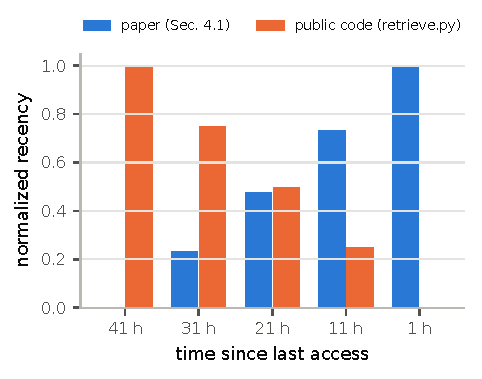
\includegraphics[width=\linewidth]{ga_recency}
\end{minipage}\hfill
\begin{minipage}{0.49\linewidth}\centering
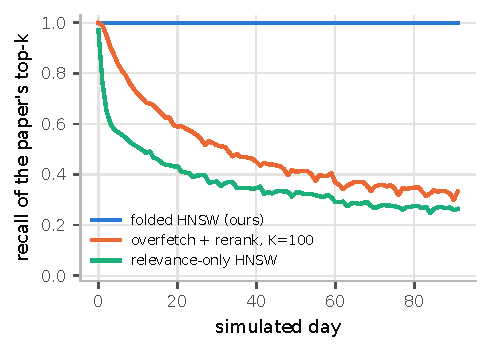
\includegraphics[width=\linewidth]{town_recall_over_time}
\end{minipage}
\caption{Left: normalised recency of five memories that differ only in their last access time, according to the paper and according to the public code. Right: recall of the paper's top-$k$ at every retrieval in the 92-day Willowbrook runs.}
\label{fig:garecency}
\end{figure}

\section{Limitations}

\begin{itemize}
\item The agents of Willowbrook follow rules where Generative Agents call a language model. This keeps the runs deterministic, free and repeatable: the town experiments in this report took \TownRuns{} runs. The comparison only needs the agents to act on what they retrieve. It also means that the size of the behavioural effects is specific to these rules. An optional script (\code{experiments/llm\_validation.py}) repeats the party scenario with planning and conversation decisions taken by a local language model.
\item Sentence embeddings come from GloVe with smooth inverse frequency weighting \citep{arora2017sif} because the machine used here cannot download neural encoders. The store is independent of the encoder.
\item The scale test attaches synthetic metadata to GloVe vectors. All timings come from a two-core virtual machine and vary by up to about 30\% between runs.
\item For a single agent's memory in the town (\TwSimMemories{} memories after 92 days) an exact scan is still faster than the folded store written in Python (\TwSimExactMs{} against \TwSimFoldedMs{} ms per retrieval). In the static benchmark the folded store is already faster at 10\,000 memories (\cref{fig:scaling}).
\item The folded index loses recall when relevance dominates the score, where plain similarity search is adequate anyway (\cref{tab:relsweep}).
\item The extension to general forgetting curves folds ACT-R's sum but not its logarithm, which changes little in the town. When every retrieval counts as a use, frequently retrieved memories crowd out new ones. Remedies are untested (\cref{sec:curvestown}). The curve uses ACT-R's usual parameters rather than values fitted to agents (\cref{sec:curvelimits}).
\end{itemize}

\section{Conclusion}

HNSW answers similarity queries. Agents ask a different question. Because recency decays exponentially, the question asked by generative agents is an inner product in disguise. A single inner-product HNSW index can answer it directly, with the weights and the time chosen per query. Making this work for a living memory takes three ingredients: time anchors with segments, a buffer for memories that were just retrieved and a cheap estimate of the normalisation ranges. The resulting store returns almost all of the paper's top-$k$ where the usual overfetch-and-re-rank pattern returns only a small part of it. In a simulated town that difference changes how far news travels and who turns up at a party. The exponential is not essential. Forgetting curves from memory research, among them ACT-R's power law over every use of a memory, are mixtures of exponentials, and eight terms of the mixture turn them into one more inner product with eight more coordinates. With a recent part scanned exactly and segments anchored after it, the coordinates stay bounded for any decay rate. The store again returns almost all of the true top-$k$, and in the town it reproduces the exact scan under ACT-R's curve as well. The forgetting model of an agent can therefore be chosen on its merits rather than on what the index can search. The town shows that this choice needs testing in a closed loop. When every retrieval counts as a use, frequently retrieved memories crowd out new ones, with or without ACT-R's logarithm. The reimplementation of HNSW reproduces the paper's parameter study except for a small gain from the hierarchy at $d=1024$. It also agrees on 100-dimensional GloVe vectors with the more recent observation that the hierarchy matters less than the neighbour heuristic.

\appendix
\section{Reproducing the results}
All code, data loaders, tests and experiment scripts are in the accompanying repository, \url{https://github.com/bogdancolceriu/agentmem-hnsw} (see \code{README.md}). The GloVe vectors are downloaded from the gensim-data release on first use. The 43 unit tests check that the folded inner product equals the score up to rounding, that with a deep search the store returns more than 99\% of the memories of the exact scan over long sequences of queries with refresh, segment compaction and min-max normalisation, that segment coordinates stay bounded and that the LangChain retriever returns at least 7 of the 8 documents of a brute-force search for every query. For the forgetting curves they also check that eight exponentials follow the three curves of \cref{tab:curvefit} within 1\%, that the bookkeeping of uses gives the same values as direct sums over whole histories, that an exponential curve of the last use gives the paper's ranking, that the Pareto fronts give the exact range of $D$, that only the exact scan accepts ACT-R's logarithm and that the folded store for general curves follows the exact scan through refresh, ageing and compaction with bounded coordinates.

\section{Use of AI tools}
This work was done with substantial help from an AI assistant (Claude, Anthropic), which wrote most of the code, ran the experiments and drafted this report. I chose the article, discussed the design of the extension with the assistant, checked the code and the results and can reproduce every experiment from the repository. Every result in the text and in the tables is generated from the result files by \code{experiments/tables.py}, so none was copied by hand.

\bibliographystyle{plainnat}
\bibliography{refs}
\end{document}
